
%%%%%%%%%%%%%%%%%%%%%%%%%%%%%%%%%%%%%%%%%%%%%%%%%%%%%%%%%%%%%%%%%%%%%%%%%%%%%%%%%%%%%%
% \section*{Notation and Conventions}
% on a pedagogical note, we would like to point out that the 4-vector $k^\mu = (\omega,\mathbf{k})$ represents the momentum and energy in the electromagnetic field while $p^{\mu}  = (E,\boldsymbol{p})$ represents the momentum and energy of plasma constituents.
% units 
% metric
% natural units 
% ecB
% eE
% ecA
% ePhi
% ct,x
% E
% pc
% mc2
% only then is c set to one

% T=perp
% L = parallel

% bf is spatial vector and cursive is 4 vector or scalar

% fourier transform definitions

%%%%%%%%%%%%%%%%%%%%%%%%%%%%%%%%%%%%%%%
%\section*{Publications and author contributions}
%\label{sec:pubs}
%\addcontentsline{toc}{chapter}{PUBLICATIONS AND AUTHOR CONTRIBUTIONS}
%%%%%%%%%%%%%%%%%%%%%%%%%%%%%%%%%%%%%%%
%Below is a list of publications from which I draw direct inspiration for the writing of this dissertation. A summary of the paper and my contributions to them are itemized.
%\begin{itemize}
%    \item \rapp{appendixA} - ``Current-conserving relativistic linear response for collisional plasmas'' by~\citet*{Formanek:2021blc} is a development of the theoretical covariant framework needed to study dense relativistic plasmas using the Vlasov-Boltzmann equation. Martin Formanek\orc{\orcD} was the lead author responsible for sections I, II, III, and the appendices that developed the covariant Vlasov-Bolztmann theory. I, Christopher Grayson \orc{\orcC}, was responsible for Section IV, which includes all figures and evaluation of the properties of the polarization tensor. Johann Rafelski\orc{\orcA} and Berndt M\"uller \orc{\orcG} were responsible for the overall direction, writing, and editing.
    
%    \item \rapp{appendixB} - ``Dynamic magnetic response of the quark-gluon plasma to electromagnetic fields'' by~\citet*{Grayson:2022asf} is a study of the dynamics of the magnetic field in quark-gluon plasma during heavy ion collisions using the ultrarelativistic limit of the theory developed in~\cite{Formanek:2021blc}. I was the lead author responsible for writing and developing theory, computation, and figures. Martin Formanek provided crosschecking, writing, and editing. Johann Rafelski and Berndt M\"uller were responsible for the overall direction, writing, and editing.

 %   \item \rapp{appendixC} - ``Electron–positron plasma in BBN: Damped-dynamic screening'' by \citet*{Grayson:2023flr} is a study of dynamic screening of the electric potential in the early universe electron-positron plasma using the non-relativistic limit of the theory developed in~\cite{Formanek:2021blc}. I was the lead author responsible for writing and developing theory, computation, and figures. Cheng Tao Yang was responsible for Section II, which evaluated the properties of the BBN plasma and overall writing and editing. Martin Formanek provided crosschecking, writing, and editing. Johann Rafelski was responsible for the overall direction, writing, and editing.
%\end{itemize}

%This dissertation includes some additional unpublished work where relevant. This line of research began in 2021 and continues to the present day. Previously, I studied strong field pair production in electromagnetic fields in heavy ion collisions, to which I hope to one day return using the knowledge I have gained in plasma physics.



%%%%%%%%%%%%%%%%%%%%%%%%%%%%%%%%%%%%%%%%%%%%%%%%%%%%%%%%%
\section{Plasma physics methods applied to Strong Fields and BBN}\label{part4}
\subsection{Plasma response to electromagnetic fields}
\label{chap:PlasmaSF}

%%%%%%%%%%%%%%%%%%%%%%%%%%%%%%%%%%%%%%%%%%%%%%%%%%%%%%%%%%%%%%%%%%%%%%%%%%%%%%%%%%%%%%
%\subsection{Linear Boltzman equation}\label{ss:BoltzPlas}
%%%%%%%%%%%%%%%%%%%%%%%%%%%%%%%%%%%%%%%%%%%%%%%%%%%%%%%%%%%%%%%%%%%%%%%%%%%%%%%%%%%%%%

% {
% \noindent 
% \centering\itshape
% The spread, both in and width and depth, of the multifarious branches of knowledge by during the last hundred odd years has confronted us with a queer dilemma. We feel clearly that we are only now beginning to acquire reliable material for welding together the sum total of all that is known into a whole; but, on the other hand, it has become next to impossible for a single mind fully to command more than a small specialized portion of it. I can see no other escape from this dilemma (lest our true who aim be lost for ever) than that some of us should venture to embark on a synthesis of facts and theories, albeit with second-hand and incomplete knowledge of some of them -and at the risk of making fools of ourselves. -Erwin Schrodinger
% }

The interaction of electromagnetic fields within relativistic plasmas is of interest in astrophysics, intense laser interactions with matter, and quark-gluon plasma in relativistic heavy ion collisions. Quark-gluon plasma (QGP), a state of matter of deconfined quarks and gluons at extremely high temperatures $T>150$ MeV, is formed in the violent collision of heavy ions at relativistic speeds. This deconfined state is also of astrophysical interest since it filled the early universe for the first few microseconds after the Big-Bang. Several methods have been introduced to study the linear response of a collisionless ultrarelativistic QGP following the seminal work by~\cite{Weldon:1982aq} by using semiclassical transport theory based on the Boltzmann equation~\cite{Mrowczynski:1987jr,Mrowczynski:1989np,Blaizot:1993zk,Kelly:1994ig,Kelly:1994dh}. However, applications of this formalism are restricted to dilute plasmas where collisions can be neglected~\cite{Blaizot:2001nr}. 
Previously, the effects of collisions within the plasma were mainly studied to derive transport coefficients, such as the electrical conductivity, of interest to the study of plasma response to long-wavelength perturbations~\cite{Mrowczynski:1988xu,Heiselberg:1993cr,Ahonen:1996nq,Baym:1997gq,Ahonen:1998iz}. In quantum field theory, transport coefficients have also been calculated using effective propagators that re-sum thermal modifications to avoid infrared divergences~\cite{Heiselberg:1994ms,Arnold:2002zm,Arnold:2003zc}. Here, we will study semi-classical transport using the Vlasov-Boltzmann equation with momentum-averaged quantum collisions between particles, a topic discussed in numerous other works, such as \cite{DeGroot:1980dk,Cercignani:2002bk,Hakim:2011bk,Carrington:2003je,Schenke:2006xu}.


The theoretical description of relativistic plasma is based on transport theory, i.e., the relativistic form of Liouville's equation. The one-particle phases space distribution function $f(x,p)$ undergoes Liouville flow,
\begin{align}
    \frac{d f(x,p)}{d\tau} = \{H(x,p), f(x,p)\} = 0\,,
\end{align}
where $p$ is the canonical four-momentum, and $x$ is the canonical position. The collision term $C[f]$ represents elastic/inelastic interactions and gives deviations away from Liouville's theorem
\begin{align}\label{eq:LpC}
    \frac{d f(x,p)}{d\tau} = C[f]\,,
\end{align}
or equivalently, entropy generation. The collision term is necessary to describe systems where the mean free path of plasma constituents is less than or equal to the characteristic length scale of the plasma or when the mean free time $\tau$ is smaller than the characteristic oscillation time of the plasma. This pertains to systems with high density, low temperature, or strongly coupled systems.

Solving the relativistic Vlasov-Boltzmann equation using the microscopic collision term \req{eq:collisionMicro} is difficult, even in the simplest cases; thus, approximate forms are often used. The relaxation-time approximation (RTA) for the collision term proposed by~\cite{Anderson:1974nyl} is a commonly made simplification to the Boltzmann equation, reducing it from an integrodifferential equation to a differential equation. The relativistic form of this collision term takes the form
\begin{equation}\label{eq:lincoll}
C[f] = (p^\mu u_\mu) \kappa [ f_\mathrm{eq}(p) - f(x,p) ] \,,
\end{equation}
where $\kappa=1/\tau$ is the relaxation rate, $f(x,p)$ is the phase space distribution of charged particles in the plasma, $f_\mathrm{eq}(p)$ is their equilibrium distribution, and $u_\mu$ is the 4-velocity of the plasma rest frame.

The RTA collision term assumes the nonequilibrium distribution $f$ returns to the equilibrium distribution in some characteristic time $\tau$, which is evident when writing \req{eq:LpC} in the form
\begin{equation}
    \frac{d f(x,p)}{dt} = \frac{f_\mathrm{eq}(p) - f(x,p) }{\tau}\,.
\end{equation}
The relaxation time $\tau$ can be computed using the schematic relaxation time approximation where an average relaxation time is introduced~\cite{Mrowczynski:1988xu,Satow:2014lia} or by calculating the momentum-dependent relaxation rate $\kappa(p)$ with the input of perturbative matrix elements~\cite{Ahonen:1996nq}. We use the average relaxation time approximation with momentum averaged $\kappa$ to make all calculations analytically tractable.

The well-known disadvantage of the RTA is that it forces all quantities, even conserved ones, to return to their equilibrium value at a rate $\tau$. This can cause the dynamics derived from this collision term to violate current and energy-momentum conservation. The violation of energy conservation is similar to introducing frictional damping into one particle Newtonian dynamics where energy is lost to the environment.
%the difference being that it neglects the dependence of friction on the velocity of particles.

Correcting for current and energy-momentum conservation is possible by adding terms that ensure that conserved quantities are unaffected~\cite{Bhatnagar:1954zz,Greene1973,Rocha:2021zcw,Singha:2023eia}. It is worth noting that this breaking of conservation law does not always affect the physical behavior of the plasma. For instance, the behavior of transverse waves in an infinite homogeneous plasma is unaffected by the addition of current conservation~\cite{Formanek:2021blc}.

In this work, we generalize the BGK modification of the linearized collision term to relativistic plasmas using the Anderson-Witting form Eq.\,(\ref{eq:lincoll}), ensuring current conservation \req{eq:collision} but not energy-momentum conservation. In \cite{Formanek:2021blc} we show that the resulting linear response functions satisfy current conservation and gauge invariance constraints. 

The preceding sections will discuss obtaining exact solutions for the covariant polarization tensor in linear response limit via Fourier transform with the BGK collision term \req{eq:collision}. We will present the plasma's electromagnetic properties by using the polarization tensor to derive the electromagnetic fields.

%%%%%%%%%%%%%%%%%%%%%%%%%%%%%%%%%%%%%%%%%%%%%%%%%%%%%%%%%%%%%%%%%%%%%%%%%%%%%%%%%%%%%%
\paragraph{Covariant kinetic theory:}\label{sec:CKT}
A full microscopic picture of plasma kinematics, useful in numerical simulations, is often more involved than what is required to understand changes in the macroscopic quantities of plasmas. A conventional simplification to the microscopic picture is to average over the discrete states to yield a distribution function $f(x,\boldsymbol{p})$, which describes the probability of finding some number of particles $dN$ in a small range of position $d\mathbf{r}^3$ and momentum $d\boldsymbol{p}^3$ or relativistically~\cite{Hakim:2011bk}
\begin{equation}
    \int_{\Sigma}d\Sigma_{\mu}\int  d^4p\frac{p^\mu}{m}f(x,p) = N,
\end{equation}
where $d\Sigma_\mu$ is the surface element on $\Sigma$
\begin{equation}
    d\Sigma_\mu = \frac{1}{3!}\epsilon_{\mu \nu \alpha\beta} dx^\nu \times dx^\alpha\times dx^\beta\,
\end{equation}
% \begin{equation}
%     dN d\tau  = f(x,p)\frac{dx^4 d^4p}{(2\pi)^4}4\pi \delta_+(p^2-m^2).
% \end{equation}
with the covariant integration, measure can be written as
\begin{equation}\label{eq:measure} 
 \frac{d^4p}{(2\pi)^4}4\pi \delta_+(p^2-m^2) = \left.\frac{d^3p}{(2\pi)^3p^0}\right|_{p^0 = \sqrt{|\boldsymbol{p}|^2 + m^2}} \,,
\end{equation}
where $p^0 = p \cdot u$ in the rest frame of the plasma. The one particle distribution function is effectively the phase space density of the system. We will always refer to the 4-momentum as $p = (p_0, \, \boldsymbol{p})$ and the 3-momentum as $\boldsymbol{p}$.

The kinetic equation describing the evolution of this distribution is the Vlasov-Boltzmann equation (VBE). The VBE is often derived in detail from heuristic arguments see \cite{DeGroot:1980dk,Cercignani:2002bk}. Here, we will outline how it relates to Liouville's theorem. A similar derivation of the equilibrium distribution in the presence of electromagnetic fields is found in \cite{Hakim:2011bk}.
We derive the classical one-species Vlasov-Boltzmann equation from the Liouville theorem
\begin{equation}
    \frac{d f(Q,P)}{d\tau} = \{H(Q,P), f(Q,P)\} = 0\,,
\end{equation}
where $P^{\mu}$ and $Q^{\mu}$ are the canonical coordinates. 
This theorem states that the canonical phase space density is conserved or the one particle phase space density $f(Q,P)$ satisfies the above continuity equation.  The Poisson bracket is explicitly written as 
\begin{equation}
    \frac{d f(Q,P)}{d\tau} = \frac{\partial Q^{\mu}}{\partial \tau}\partial_\mu f(Q,P) + \frac{\partial P^{\mu}}{\partial \tau}\frac{\partial f(Q,P)}{\partial P^{\mu}}\,.
\end{equation}
Since we consider these particles in the presence of electromagnetic fields, we use the relativistic EM Hamiltonian in the Bergmann form
\begin{equation}
    H(Q,P) = \sqrt{(P-q A(Q))_\mu(P-q A(Q))^\mu}\,,
\end{equation}
which contracts the kinetic momentum to give the relativistic energy of a particle in an electromagnetic field. The equations of motion are
\begin{align}
    \frac{\partial Q^{\mu}}{\partial \tau} &= \frac{\partial H(Q,P)}{\partial P_{\mu}}= \frac{(P-q A(Q))^{\mu}}{H(Q,P)}\,,\\
   -\frac{\partial P^{\mu}}{\partial \tau} &= \frac{\partial H(Q,P)}{\partial Q^{\mu}}= - \frac{(P-q A(Q))^{\nu}q \partial_\mu A_\nu(Q)}{H(Q,P)}\,.
\end{align}
If a canonical transformation is applied to our coordinates, the Liouville theorem states that the phase space density remains unchanged. 
The transformation we would like to consider is the transition from kinetic to canonical coordinates where $Q^{\mu}\rightarrow x^{\mu}$ and  $P^{\nu} \rightarrow P^{\nu} - q A^{\nu}(x)$. This new momentum is related to the actual velocity of the particle $P^{\nu} - q A^{\nu}(x) = p^{\mu} = m\frac{d x^{\mu}}{d \tau}$.  We then consider the Liouville theorem for the shifted function,  
\begin{equation}
 \frac{d x^{\mu}}{d \tau}\partial_\mu f(x,P-q A(x)) + \frac{d (P-q A(x))^{\mu}}{d \tau}\frac{\partial f(x,P-q A(x))}{\partial (P-q A(x))^{\mu}}\,.
\end{equation}
Then, we use the equations of motion to write
\begin{equation}
    \frac{(P-q A(x))^{\mu}}{H(x,P)} \partial_\mu f(x,P-q A(x)) + q\frac{(P-q A(x))_{\nu}}{H(x,P)} F^{\mu \nu}(x) \frac{\partial f(x,P-q A(x))}{\partial (P-q A(x))^{\mu}}\,.
\end{equation}
Where the electromagnetic tensor is $F^{\mu \nu} = \partial^{\mu} A^{\nu}  - \partial^{\nu}A^{\mu}$. 
Since the canonical momentum is related to the kinetic momentum by $ P^{\mu}  = m\frac{d x^{\mu}}{d \tau} + q A^{\mu}(x)$, we rewrite the Liouville flow in terms of kinetic momentum $p^\mu = m \frac{dx^\mu}{d\tau}$. Applying Liouville's theorem allows us to set the whole expression to zero to recover the collisionless Vlasov-Boltzmann equation
\begin{equation}
    p^{\mu} \partial_\mu f(x, p) + q  p_{\nu} F^{\mu \nu}(x) \frac{\partial f(x, p )}{\partial  p^{\mu} }=0
\end{equation}
where $ p^{\mu} = m\frac{d x^{\mu}}{d \tau}$. The collision term is then added to allow for deviations from constant phase space density flow
\begin{equation}\label{eq:VBE}
\boxed{(p_k \cdot \partial) f_k(x,p_k) + q_k F^{\mu\nu} p^k_\nu \frac{\partial f_k(x,p_k)}{\partial p_k^\mu} =\sum_l \, (p_k\cdot u)C_{kl}(x,p_k)}\,,
\end{equation}
where there are $k$ equations for each particle species and a $l$ sum over all possible collisions with particle $k$. Usually, we drop the subscript $k$ on momentum if there is no ambiguity. The first term describes the flow or diffusion of particles in the medium, the second term generates an electromagnetic force on particles, and the collision term is on the right-hand side. Generally, each plasma constituent will have a Boltzmann equation and collisions between each species. The collision term represents the detailed microscopic scattering between the plasma constituents. The collision term for the reaction $k+l\rightarrow i+j$ is defined as
\begin{equation}\label{eq:collisionMicro}
    C_{kl}(x,p_k) = \frac{1}{2}\sum^N_{i=1}\sum^N_{j=1}\int \frac{d^3p_l}{(2 \pi)^3p_l^0}\frac{d^3p_i}{(2 \pi)^3p_i^0}\frac{d^3p_j}{(2 \pi)^3p_j^0}\left[f_if_j -f_k f_l
    \right]W_{kl|ij}\,,
\end{equation}
where 
$k,l = 1,2,...,N$ and $W_{ij|kl}$ is the transition rate for the respective collision.
It is important to note that in this framework for a plasma forced by external fields, the collision term is the only way a particle species can impact the dynamics of the phase space distribution of another species.

\paragraph{The BGK collision term}
As discussed previously the integral in \req{eq:collisionMicro} vastly complicates solving the Vlasov-Boltzmann equation. Instead, we will use a simplified collision term that returns the distribution $f(x,p)$ to equilibrium at some characteristic rate $\kappa = 1/\tau$, reducing \req{eq:VBE} from an integro-differential equation to a differential equation. The relaxation rate or damping rate $\kappa$ is the sum of all possible collisions~\cite{Das:2021bkz}
\begin{equation}
    \kappa_k(p) = \sum^N_{i=1}\sum^N_{j=1}\sum^N_{l=1} \frac{1}{2}\int\frac{d^3p_l}{(2 \pi)^3p_l^0}\frac{d^3p_i}{(2 \pi)^3p_i^0}\frac{d^3p_j}{(2 \pi)^3p_j^0}f_l^{\text{eq}}W_{kl|ij}\,
\end{equation}
In \cite{Formanek:2021blc} we utilize the simplified collision term proposed by Ref.~\cite{Bhatnagar:1954zz} (BGK), which is amended to conserve the current 
\begin{equation}\label{eq:collision}
    \boxed{C(x,p) =\kappa\left(f_{\text{eq}}(p)\frac{n(x)}{{n_{\text{eq}}}} - f(x,p)\right)}\,,
\end{equation}
The non-equilibrium and equilibrium densities are defined covariantly as
\begin{align}
\label{eq:ndef1}n(x) &\equiv 2 \int \frac{d^3p}{(2\pi)^3p^0}(p \cdot u)f(x,p)\,,\\
\label{eq:ndef2}n_\mathrm{eq} &\equiv 2\int \frac{d^3p}{(2\pi)^3p^0}(p \cdot u) f_\mathrm{eq}(p)\,.
\end{align}
The factor of two accounts for the spin degrees of freedom. This correction is also proposed in \cite{Rocha:2021zcw} where they treat the collision term as an operator adding counterterms to ensure that when acting on conserved quantities like energy, momentum, and particle number, the modified collision operator yields zero, thereby respecting the fundamental conservation laws. We can see that \req{eq:collision} explicitly conserves the 4-current~\cite{Formanek:2021blc}
\begin{equation}\label{eq:jmudef}
j_{\mathrm{ind}}^\mu (x)= 2q \int \frac{d^3p}{(2\pi)^3p^0}p^\mu f(x,p)\,,
\end{equation}
by applying $\partial_\mu$ on this expression and substituting back from the Boltzmann equation \req{eq:boltzmanncov}
\begin{equation}
\partial_\mu j^\mu = 2q \int \frac{d^3p}{(2\pi)^3p^0} \left\{-q F^{\mu\nu}p_\nu \frac{\partial f(x,p)}{\partial p^\mu}\right. 
\left. + (p \cdot u)\kappa \left[f_\mathrm{eq}(p) \frac{n(x)}{n_\mathrm{eq}}-f(x,p) \right] \right\}\,.
\end{equation} 
The first term should naturally vanish because the collisionless Vlasov equation preserves 4-current. This can be seen upon integration by parts and use of the antisymmetry of $F^{\mu\nu}$. On the other hand, the collision term vanishes by design - see definitions (\ref{eq:ndef1},\ref{eq:ndef2}). This is in contrast to the Anderson-witting collision term, which does not conserve current \req{eq:lincoll}.


%%%%%%%%%%%%%%%%%%%%%%%%%%%%%%%%%%%%%%%%%%%%%%%%%%%%%%%%%%%%%%%%%%%%%%%%%%%%%%%%%%%%%%
%~~~~~~~~~~~~~~~~~~~~~~~~~~~~~~~~~~~~~~~~~~~~~~~~~~~~~~~~~~~~~~~~~~~~~~~~~~~~~~~~~~~~~~~~~~~~~~~~
\subsection{Linear response: electron-positron plasma}
The transport properties of electron-positron plasma are governed by three Vlasov-Boltzmann equations \cite{Grayson:2023flr}
\begin{align}\label{eq:VBEf}
(p \cdot \partial) f_\pm(x,p) + &q F^{\mu\nu} p_\nu \frac{\partial f_\pm(x,p)}{\partial p^\mu} = C_\pm(x,p)\,,\\
\label{eq:VBEg}(p \cdot \partial) f_\gamma(x,p) &= C_\gamma(x,p)\,.
\end{align}
The subscripts $-$, $+$, and $\gamma$ indicate the transport equation for electrons, positrons, and photons. These form a system of differential equations for each distribution function $f_i(x,p)$. We suppress the 4-momentum subscript for each species $f_i(x,p) = f_i(x,p_i)$ to simplify notation. 

Since photons cannot couple directly to the electromagnetic field, they do not contribute to the dynamics of the electromagnetic field at first-order polarization response as indicated in Eq.\,(\ref{eq:VBEg}). This is not true for a QCD plasma where gluons could couple directly to an external gluon field.

To find the effect of electrons and positrons on the electromagnetic fields, we use the transport equations \req{eq:VBEf} to find the induced current in the plasma
\begin{equation}
j_{\mathrm{ind}}^\mu(x) = 2\int \frac{d^3 p}{(2 \pi)^3 p^0}p^\mu \left[f_+(x,p)-f_-(x,p)\right]\,,
\end{equation}
found via Fourier transformation and related to the induced current in the linear response equation
\begin{equation}
    \widetilde{j}_{\mathrm{ind}}^{\mu}(k) = {\Pi^{\mu}}_{\nu}(k) \widetilde{A}^{\nu}(k)\,,
\end{equation}
to identify the polarization tensor $\Pi^{\mu}_{\nu}$. To begin, we solve the Vlasov-Boltzmann equation with the BGK collision term
\begin{equation}\label{eq:boltzmanncov}
(p \cdot \partial) f_\pm(x,p) + q F^{\mu\nu} p_\nu \frac{\partial f_\pm(x,p)}{\partial p^\mu} = (p \cdot u)\kappa_\pm\left[f^\mathrm{eq}_\pm(p)\frac{n_\pm(x)}{n^\mathrm{eq}_\pm} - f_\pm(x,p)\right]\,.
\end{equation}
Since the solutions for these equations will differ only by the sign of charge, we need only solve one to understand dynamics. The $\pm$, which indicates electrons or positrons, may be dropped when unnecessary in the equations below.

We assume for the equilibrium distribution the covariant Fermi-Dirac distribution function~\cite{DeGroot:1980dk,Hakim:1967prd}:
\begin{equation}\label{eq:fb}
f^\mathrm{eq}_\pm(x,p) \equiv \frac{1}{e^{([p^{\mu} +q A^\mu (x) ] u_\mu\pm \mu_q)/T} + 1}\,,
\end{equation}
where $p^\mu+q A^\mu (x)$ is the canonical momentum in the presence of an electromagnetic 4-potential, $u^\mu$ is the global 4-velocity of the medium, $T$ denotes the temperature in the medium rest frame, and $\mu_q$ is the chemical potential related to charge. 

The linear response approximation assumes the distribution function can be written as a sum of the equilibrium distribution $f_\mathrm{eq}(x,p)$ plus a small perturbation away from the equilibrium $\delta f(x,p)$
\begin{equation}\label{eq:perturbation}
f(x,p) = f_\mathrm{eq}(x,p) + \delta f(x,p)\,.
\end{equation}
Here the small perturbation $\delta f(x,p)$ is induced by an external electromagnetic field. We expand \req{eq:boltzmanncov} in equilibrium and perturbation terms \cite{melrose2008quantum}
\begin{multline}
    (p \cdot \partial)\left(f_\mathrm{eq}(x,p)+ \delta f(x,p)\right) +  q \left(F_{\mathrm{eq}}^{\mu\nu} +\delta F^{\mu\nu}\right)p_\nu \frac{\partial (f_\mathrm{eq}(x,p)+\delta f(x,p))}{\partial p^\mu} \\ = \kappa (p\cdot u)\left(f_\mathrm{eq} (p)\frac{\delta n(x)}{{n_\mathrm{eq}(x)}} - \delta f(x,p)\right)\,.
\end{multline}
Since the equilibrium expressions are a solution to the collisionless Boltzmann equation, all the equilibrium terms combined are zero. The collision term is constructed to be zero at equilibrium. We will neglect the Lorentz force due to the induced field on the perturbation since it is second order in the perturbation
\begin{equation}
    (p \cdot \partial) \delta f(x,p)+ q \delta F^{\mu\nu}p_\nu \frac{\partial f(x,p)}{\partial p^\mu} = \kappa (p\cdot u)\left(f_{\text{eq}} (x,p)\frac{\delta n(x)}{{n_{\text{eq}}(x)}} - \delta f(x,p)\right)\,.
\end{equation}
where the quantity $\delta n(x)$ is defined following the definitions(\ref{eq:ndef1},\ref{eq:ndef2}) as
\begin{equation}
\delta n (x) \equiv 2 \int \frac{d^3p}{(2\pi)^3p^0} (p \cdot u)\delta f(x,p)\,.
\end{equation}
At this point, we will take the weak field limit of the equilibrium distribution, which assumes the change in energy of a particle due to the electromagnetic field is small in comparison to the thermal energy
\begin{equation}
    \frac{ qA(x)\cdot u}{T}\ll 1\,.
\end{equation}
In this case, the equilibrium distribution becomes the usual
\begin{equation}\label{eq:equilibriumFD}
f^\mathrm{eq}_\pm(x,p) \equiv \frac{1}{e^{(p^{\mu}  u_\mu\pm \mu_q)/T} + 1}\,.
\end{equation}
An explicit solution of the Vlasov-Boltzmann equation can be obtained more easily in momentum space after a Fourier transformation.  We define the Fourier transform $\widetilde{g}(k^\mu)$ of a general function $g(x^\mu)$ of space-time coordinates as 

\begin{equation}\label{eq:ftdef}
g(x) = \int \frac{d^4k}{(2\pi)^4} \, e^{-i k \cdot x} \, \widetilde{g}(k)\,.
\end{equation} 
The Fourier transformation replaces partial derivatives $\partial_\mu$ with the 4-momentum $k_\mu$:
\begin{equation}
\partial_\mu \rightarrow - i k_\mu \,.
\end{equation}
The 4-vector $k^\mu = (\omega,\mathbf{k})$ represents the momentum and energy in the electromagnetic field. In contrast, $p^{\mu}  = (E,\boldsymbol{p})$ represents the momentum and energy of plasma constituents.

Using these definitions, the Fourier-transformed Boltzmann equation reads \cite{Formanek:2021blc}
\begin{equation}\label{eq:boltzfourier}
-i (p \cdot k) \widetilde{\delta f}(k,p) + q\widetilde{F}^{\mu\nu}p_\nu \frac{\partial f_\mathrm{eq}(p)}{\partial p^\mu} 
= (p \cdot u)\kappa \left[\frac{f_\mathrm{eq}(p)}{n_\mathrm{eq}}\widetilde{\delta n}(k) - \widetilde{\delta f}(k,p) \right]\,.
\end{equation}
In the following, we simplify the notation of derivatives of the equilibrium function with respect to momentum as
\begin{equation}
\frac{\partial f_\mathrm{eq}(p)}{\partial p^\mu} = \frac{d f_\mathrm{eq}(p)}{d (p \cdot u)} u_\mu \equiv f'_\mathrm{eq}(p) u_\mu \,.
\end{equation}
We solve \req{eq:boltzfourier} for the perturbation $\widetilde{\delta f}(k,p)$, which describes fluctuations away from equilibrium due to the electromagnetic field
\begin{equation}\label{eq:deltaftilde}
\widetilde{\delta f}(k,p) = \frac{i}{p \cdot k + i (p \cdot u) \kappa}\bigg[-q (u \cdot \widetilde{F} \cdot p)f'_\mathrm{eq}(p) 
\left.+ (p \cdot u) \kappa \frac{f_\mathrm{eq}(p)}{n_\mathrm{eq}}\widetilde{\delta n}(k)\right]\,.
\end{equation}
This can be readily integrated to obtain an equation for $\widetilde{\delta n}(k)$
\begin{equation}
\widetilde{\delta n}(k) = R(k) - Q(k)\widetilde{\delta n}(k)\,,
\end{equation}
where the integrals are defined as
\begin{align}\label{eq:R}
R(k)  \equiv -2i \int \frac{d^3p}{(2\pi)^3p^0}(p \cdot u) \frac{q(u \cdot \widetilde{F} \cdot p)f'_\mathrm{eq}}{p \cdot k + i (p \cdot u)\kappa}\,,\\
\label{eq:Q}Q(k) \equiv -2i \frac{\kappa}{n_\mathrm{eq}}\int \frac{d^3p}{(2\pi)^3p^0}(p \cdot u)^2 \frac{f_\mathrm{eq}(p)}{p\cdot k + i(p \cdot u)\kappa}\,.
\end{align}
The solution for $\widetilde{\delta n}(k)$ in terms of the external fields is simply 
\begin{equation}
\widetilde{\delta n}(k) = \frac{R(k)}{1+Q(k)}\,.
\end{equation}
We can substitute this result back into (\ref{eq:deltaftilde}) to obtain an explicit expression for $\widetilde{\delta f}(k,p)$ found in \cite{Formanek:2021blc}
\begin{equation}\label{eq:deltafsolution}
	\widetilde{\delta f}(k,p) = \frac{i}{p \cdot k + i (p \cdot u) \kappa}\bigg[-q (u \cdot \widetilde{F} \cdot p)f'_\mathrm{eq}(p) 
	\left.+ (p \cdot u) \kappa \frac{f_\mathrm{eq}(p)}{n_\mathrm{eq}} \frac{R(k)}{1+Q(k)}\right]\,.
\end{equation}
The right-hand side contains only known quantities. In the next section, we will use \req{eq:deltafsolution} to calculate the induced current in the plasma. Adding additional conservation laws requires further integrals to solve the Vlasov-Boltzmann equation involving higher moments of the fluctuation $\delta f$ as discussed in \cite{Rocha:2021zcw,Singha:2023eia}.

%=====================================================================
\paragraph{Induced current:}

The induced charge current is the sum of the antiparticle distribution $\widetilde{f}_-$ and the particle distribution $\widetilde{f}_+$
\begin{equation}\label{eq:perturbation1}
\tilde{j}_{\mathrm{ind}}^\mu(k) = 2\int \frac{d^3 p}{(2 \pi)^3 p^0}p^\mu 
\sum_{i = \, +, \, -} q_i \tilde{f}_{i}(k,p)\,,
\end{equation}
with the factor of two accounting for spin. Sometimes, this is referred to as the first moment of $\delta f$.
After expanding in linear response \req{eq:perturbation}, and specifying $q_\pm = \pm e$ the induced current is a function of the perturbation
\begin{align}\label{eq:perturbation2}
\tilde{j}_{\mathrm{ind}}^\mu(k) = 2\int \frac{d^3 p}{(2 \pi)^3 p^0}p^\mu \Big( e \left[\tilde{f}^{\mathrm{eq}}_+(k,p)-\tilde{f}^{\mathrm{eq}}_-(k,p)\right]\notag\\
+ e\left[\delta\tilde{f}_+(k,p)-\delta\tilde{f}_-(k,p)\right]
\Big)
\notag\\
=4 e\int \frac{d^3 p}{(2 \pi)^3 p^0}p^\mu \delta\tilde{f}(k,p)
\,.
\end{align}
The equilibrium currents cancel in the weak field limit for zero chemical potential, and the perturbations add since they differ by the charge $\delta f_\pm=\pm e \delta f' $. For finite chemical potential $\mu_q$, the equilibrium terms can be combined with hyperbolic trig-identities
\begin{equation}
\begin{split}
\tilde{j}_{\mathrm{ind}}^\mu(k) 
=2 e\int \frac{d^3 p}{(2 \pi)^3 p^0}p^\mu \Big(&-\frac{\sinh{(\mu_q)}}{\cosh{(p \cdot u)}+\cosh{(\mu_q)}} \\&+  \left[\delta\tilde{f}_+(k,p)-\delta\tilde{f}_-(k,p)\right]
 \Big)
\,.
\end{split}
\end{equation}
For now, we will focus on the case of zero chemical potential, $\mu_q=0$, where the first term vanishes.
We can express the induced current in terms of defined integrals \cite{Formanek:2021blc} resulting from inserting \req{eq:deltafsolution} into the induced current
\begin{equation}\label{eq:jmu}
\widetilde{j}_{\mathrm{ind}}^\mu(k) = R^\mu(k) - \frac{R(k)}{1+Q(k)} Q^\mu(k)
\end{equation}
where the integrals $R^\mu(k)$ and $Q^\mu(k)$ are defined analogously to (\ref{eq:R},\ref{eq:Q}) as
\begin{align}
\label{eq:Rmu}R^\mu(k)  \equiv -4q^2i \int \frac{d^3p}{(2\pi)^3p^0} p^\mu \frac{(u \cdot \widetilde{F} \cdot p)f'_\mathrm{eq}}{p \cdot k + i (p \cdot u)\kappa}\,,\\
\label{eq:Qmu}Q^\mu(k) \equiv -4qi \frac{\kappa}{n_\mathrm{eq}}\int \frac{d^3p}{(2\pi)^3p^0}(p\cdot u) p^\mu \frac{f_\mathrm{eq}(p)}{p\cdot k + i(p \cdot u)\kappa}\,.
\end{align} 
Note that we absorbed the factor $4e$ from the current (\ref{eq:perturbation2}) into the definition of these integrals. The $R^{\mu}$ term is what one would find from the collisionless case $\kappa \rightarrow 0^+$. The induced current for the normal RTA collision term, which does not conserve current, is obtained by setting $\delta n \rightarrow n_{eq}$ or equivalently
\begin{equation}\label{eq:jRTA}
\widetilde{j}_{\mathrm{AW}}^\mu(k) = R^\mu(k) - Q^\mu(k)
\end{equation}

% %=====================================================================
% \subsection{Current conservation}

% We can show that the result (\ref{eq:jmu}) satisfies the continuity equation. In the momentum space this expression has to be orthogonal to $k_\mu$. The first term
% \begin{equation}
% k_\mu R^\mu = -4q^2i \int \frac{d^3p}{(2\pi)^3p^0} [k \cdot p + i(p \cdot u)\kappa - i(p \cdot u)\kappa)]
% \times  \frac{(u \cdot \widetilde{F} \cdot p)f'_\mathrm{eq}}{p \cdot k + i (p \cdot u)\kappa} = -i2q\kappa R\,,
% \end{equation}
% where we added and subtracted $i (p \cdot u)\kappa$ in the numerator. The integral for which the denominator cancels vanishes. On the other hand
% \begin{equation}
% k_\mu Q^\mu = -4qi \frac{\kappa}{n_\mathrm{eq}}\int \frac{d^3p}{(2\pi)^3p^0} [k \cdot p + i(p \cdot u)\kappa - i(p \cdot u)\kappa)]
% \times \frac{(p \cdot u)f_\mathrm{eq}(p)}{p\cdot k + i(p \cdot u)\kappa} = - 2qi\kappa(1+Q)\,,
% \end{equation}
% because the part where the denominator cancels integrates to $n_\mathrm{eq}$ by definition (\ref{eq:ndef2}). Substituting all into our result (\ref{eq:jmu}) we have
% \begin{equation}
% k \cdot \widetilde{j}(k) = -i2q\kappa R + \frac{R2qi\kappa}{1+Q}(1+Q)=0\,,
% \end{equation}
% as expected.

% %======================================================================
\paragraph{Covariant polarization tensor:}

To find the polarization tensor, we compare our result (\ref{eq:jmu}) to the covariant formulation of Ohm's law~\cite{Starke:2014tfa} which both describe the induced current in the momentum space
\begin{equation}\label{eq:ohm}
\widetilde{j}^\mu(k) = \Pi^\mu_\nu(k) \widetilde{A}^\nu(k)\,.
\end{equation}
To perform this comparison and extract the polarization tensor we must rewrite the Fourier transform of the electromagnetic tensor in terms of the 4-vector potential in momentum space $\widetilde{A}^\mu(k)$
\begin{equation}\label{eq:ftfmunu}
\widetilde{F}^{\mu\nu}(k) = -i k^\mu \widetilde{A}^\nu(k) + i k^\nu \widetilde{A}^\mu(k)\,.
\end{equation}
We then substitute this into the definition of $R^\mu(k)$ (\ref{eq:Rmu}) and isolate $\widetilde{A}^\mu$ as so it is in the form of \req{eq:ohm} to obtain \cite{Formanek:2021blc}
\begin{equation}
R^\mu(k) = - 4q^2 \int \frac{d^3p}{(2\pi)^3p^0} f'_\mathrm{eq}(p)
\times \frac{(u\cdot k)p^\mu p_\nu - (k \cdot p)p^\mu u_\nu}{p\cdot k + i (p \cdot u) \kappa} \widetilde{A}^\nu(k)\,,
\end{equation}
from which we see that the contribution of $R^\mu$ to the polarization tensor is
\begin{equation}\label{eq:Rmunu}
R^\mu_\nu(k) \equiv - 4q^2 \int \frac{d^3p}{(2\pi)^3p^0} f'_\mathrm{eq}(p)
\times\frac{(u\cdot k)p^\mu p_\nu - (k \cdot p)p^\mu u_\nu}{p\cdot k + i (p \cdot u) \kappa}.
\end{equation}
The contribution of the second term is hidden in the $R(k)$ scalar. In terms of the 4-vector potential in the momentum space $\widetilde{A}^\nu$ we have
\begin{equation}
R(k) = - 2q \int \frac{d^3p}{(2\pi)^3p^0}(p \cdot u)f'_\mathrm{eq}(p)
\times\frac{(u\cdot k)p_\nu - (k \cdot p)u_\nu}{p\cdot k + i (p \cdot u) \kappa}\widetilde{A}^\nu(k)\,.
\end{equation}
We can identify in this expression a 4-vector $H_\nu(k)$ defined as
\begin{equation}\label{eq:Hnu}
H_\nu(k) \equiv - 2q \int \frac{d^3p}{(2\pi)^3p^0}(p \cdot u)f'_\mathrm{eq}(p)
\times\frac{(u\cdot k)p_\nu - (k \cdot p)u_\nu}{p\cdot k + i (p \cdot u) \kappa}
\end{equation}
so that the polarization tensor is given by
\begin{equation}\label{eq:pimunu}
\boxed{\Pi^\mu_\nu(k) = R^\mu_\nu(k) - \frac{Q^\mu(k) H_\nu(k)}{1+Q(k)},}
\end{equation}
where the covariant quantities $R^\mu_\nu$, $Q^\mu$, $H_\nu$, and $Q$ are given by the integrals (\ref{eq:Rmunu}, \ref{eq:Qmu}, \ref{eq:Hnu}, \ref{eq:Q}) respectively. 
This is the final covariant form of the current conserving covariant polarization tensor for an infinite homogeneous plasma. The bulk of the work in applying \req{eq:pimunu} to a specific scenario is choosing an equilibrium distribution and evaluating the integrals. Explicit expressions for the components of this tensor in the rest frame of the plasma are found in the ultrarelativistic limit \req{eq:polfuncsUltra} and in the non-relativistic limit \req{eq:polfuncs} in \cite{Formanek:2021blc}.
This polarization tensor is also derived in \cite{Carrington:2003je} and \cite{Schenke:2006xu}. The correction to the polarization tensor found by using the collision term with current conservation \req{eq:collision} is given by the second term in \req{eq:pimunu}. The current conserving correction modifies the longitudinal polarization properties of the tensor related to charge fluctuations but not the transverse properties related to electromagnetic waves. The Anderson-Witting form of the polarization tensor found using the collision term \req{eq:lincoll} is equivalent to $R^\mu_\nu$ and the polarization tensor for a collisionless plasma is $R^\mu_\nu$ with $\kappa \rightarrow 0^+$.



% We briefly mention the properties of the polarization tensor. The induced charges have to satisfy the continuity equation; in momentum space this implies
% \begin{equation}\label{eq:currentconserv}
% k_\mu \widetilde{j}^\mu = 0 = k_\mu \Pi^\mu_\nu \widetilde{A}^\nu\,.
% \end{equation}
% Since the current also has to be gauge invariant
% \begin{equation}\label{eq:transversal2}
% \left.
% \begin{array}{c}
% \widetilde{j}'^\mu_\text{ind} = \Pi^\mu_\nu \widetilde{A}'^\nu = \Pi^\mu_\nu (\widetilde{A}^\nu - i k^\nu \widetilde{\chi}),\\
% \widetilde{j}^\mu_\text{ind} = \Pi^\mu_\nu \widetilde{A}^\nu
% \end{array}
% \right\} \ \Rightarrow \Pi^\mu_\nu k^\nu = 0\,,
% \end{equation}
% where $\widetilde{\chi}(k)$ is a Fourier transform of an arbitrary gauge function. This implies that if we multiply the polarization tensor from the right with $k^\nu$ it should vanish. This property is apparent in the covariant form of $H_\nu(k)$ (\ref{eq:Hnu}) and $R^\mu_\nu(k)$ (\ref{eq:Rmunu}). 

\subsection{Self-consistent electromagnetic fields in a medium}\label{sec:Maxwell}
To find the electromagnetic field in a plasma, we solve Maxwell's equations self-consistently in an infinite homogeneous and stationary polarizable medium. In this medium, Maxwell's equations take on the usual form \cite{melrose2008quantum}
\begin{equation}
\partial^{[\mu}F^{\nu \rho]}(x) =0, \quad \partial_{\mu}F^{\mu \nu}(x) = \mu_0 J^{\nu}(x)\,,
\end{equation}
Using the Fourier transform defined as in equation \req{eq:ftdef} we replace partial derivatives $\partial_\mu$ with the 4-momentum $-i k_\mu$. Then Maxwell's equations in Fourier space are
\begin{equation}
-i k^{[\mu}\widetilde{F}^{\nu \rho]}(k) =0, \quad -i k_{\mu}\widetilde{F}^{\mu \nu}(k) = \mu_0 \widetilde{J}^{\nu}(k)\,,
\end{equation}
$k=(\omega, \boldsymbol{k})$ is the 4-wavevector of the electromagnetic field. The properties of the medium are introduced by writing the 4-current $\widetilde{J}^{\mu}$ in terms of its induced and external parts
\begin{equation}
 \widetilde{J}^{\mu}(k) = \widetilde{j}_{\mathrm{ext}}^{\mu}(k)+ \widetilde{j}_{\mathrm{ind}}^{\mu}(k)\,.
\end{equation}
The induced current $\widetilde{j}_{\mathrm{ind}}^{\mu}$, to leading order, is given by the polarization tensor through \req{eq:ohm}. Though the induced current is linear with respect to the self-consistent field $\widetilde{A}^{\nu}$, the field itself is intrinsically nonlinear regarding plasma response as we shall see when solving for the self-consistent fields \reqs{eq:phi}{eq:aperp}. Nonlinear response comes from higher-order terms involving nested convolution integrals of the polarization tensor and the self-consistent potential and is required when the polarization current is on the order of the external current.

Solving Maxwell's equations in the Lorentz gauge $k \cdot \widetilde{A}=0$ one finds the usual expression
\begin{equation}\label{eq:Amu}
\begin{split}
\widetilde{A}^{\mu}(k)&= -\frac{\mu_0}{k^2}\left(\widetilde{j}_{\mathrm{ext}}^{\mu}(k)+ \widetilde{j}_{\mathrm{ind}}^{\mu}(k)\right)\\
&= -\frac{\mu_0}{k^2}\left(\widetilde{j}_{\mathrm{ext}}^{\mu}(k)+  \Pi^\mu_\nu(k) \widetilde{A}^\nu(k)\right)\,,
\end{split}
\end{equation}
$\mu_0$ denotes the magnetic permittivity of the vacuum, and we have used \req{eq:ohm} to express the induced current. 

\paragraph{Projection of plasma polarization tensor.} We proceed by algebraically solving for the self-consistent potential. To do this, we first note that in a homogeneous medium, the response depends only on two independent scalar polarization functions $\Pi_\parallel$ and $\Pi_\perp$ describing polarization in the parallel and transverse directions relative to the wave-vector $\boldsymbol{k}$ \cite{Weldon:1982aq}. The polarization tensor may be written in terms of these polarization functions as
\begin{equation}\label{eq:poltensgen}
 \Pi^{\mu \nu}(k,u) = \Pi_\parallel(k) L^{\mu \nu}(k,u) + \Pi_\perp(k) S^{\mu \nu}(k,u)\,,
\end{equation}
where $k^\mu$ is the 4-momentum of the field and $u^\mu$ is the 4-velocity of the medium. The polarization tensor represents the electromagnetic response of the medium to the electromagnetic field. $\Pi_\parallel$ usually describes charge fluctuations and $\Pi_\perp$ describes the properties of electromagnetic waves. For optically active or chiral mediums there is also a rotational portion of the polarization tensor $\Pi_R$. Since we neglect spin, our derivation of the polarization tensor is not sensitive to $\Pi_R$. Conventions for the longitudinal and transverse projection tensors, $L^{\mu \nu}$ and  $S^{\mu \nu}$, may be found in \cite{melrose2008quantum}. These tensors are reproduced here for convenience
\begin{equation}
     L^{\mu \nu} \equiv \frac{k^2}{(k\cdot u)^2-k^2}\bigg[ \frac{ k^{\mu}u^{\nu}}{(k\cdot u)}+ \frac{ k^{\nu}u^{\mu}}{(k\cdot u)} -\frac{k^2u^{\mu}u^{\nu}}{(k\cdot u)^2}  -\frac{k^{\mu}k^{\nu}}{k^2} \bigg]\,,
\end{equation}
\begin{equation}
     S^{\mu \nu} \equiv g^{\mu \nu} +\frac{1}{(k\cdot u)^2-k^2}\bigg[ k^{\mu}k^{\nu} 
     -(k\cdot u)( k^{\mu}u^{\nu}+k^{\nu}u^{\mu})+k^2u^{\mu}u^{\nu}\bigg]\,.
\end{equation}
These projections are equivalent to ones defined in \cite{Weldon:1982aq} up to an overall normalization. To simplify the calculation, the wave-vector $\boldsymbol{k}$ is chosen, without loss of generality, to point along the third spatial direction ($\mu=3$):
 \begin{equation}\label{eq:poltenmat}
    \Pi^{\mu}_{\nu}(\omega,\boldsymbol{k}) = \left[
    \begin{array}{cccc}
-\frac{|\mathbf{k}|^2}{\omega^2}\Pi_{\parallel}& 0 & 0 & \frac{|\mathbf{k}|}{\omega}\Pi_{\parallel} \\
 0 & \Pi_{\perp} & 0 & 0 \\
 0 & 0 & \Pi_{\perp} & 0 \\
 -\frac{|\mathbf{k}|}{\omega}\Pi_{\parallel} & 0 & 0 & \Pi_{\parallel} \\ 
\end{array}
\right]\,.
\end{equation}
Utilizing this decomposition, we can immediately see that the transverse polarization function will be related to the $\Pi^1_1 = \Pi^2_2 = \Pi_\perp$ component of the polarization tensor defined in \req{eq:pimunu}. Analogously the longitudinal portion of the polarization tensor is given by calculating the $\Pi^3_3 = \Pi_\parallel$ component. The spatial component of the potential $\widetilde{\boldsymbol{A}}$  in these coordinates can be expressed as
\begin{equation}
\widetilde{\boldsymbol{A}} = \widetilde{A}_\parallel \hat{\boldsymbol{k}} + \widetilde{\boldsymbol{A}}_\perp\,,
\end{equation}
which implies
\begin{equation}
 \widetilde{A}_{\parallel} = \frac{\boldsymbol{k} \cdot  \widetilde{\boldsymbol{A}}}{|\boldsymbol{k}|}, \quad   \widetilde{\boldsymbol{A}}_{\perp} = \widetilde{\boldsymbol{A}} -  \widetilde{A}_{\parallel}\hat{\boldsymbol{k}}\,,
\end{equation}
\begin{figure}[h!]
    \centering
    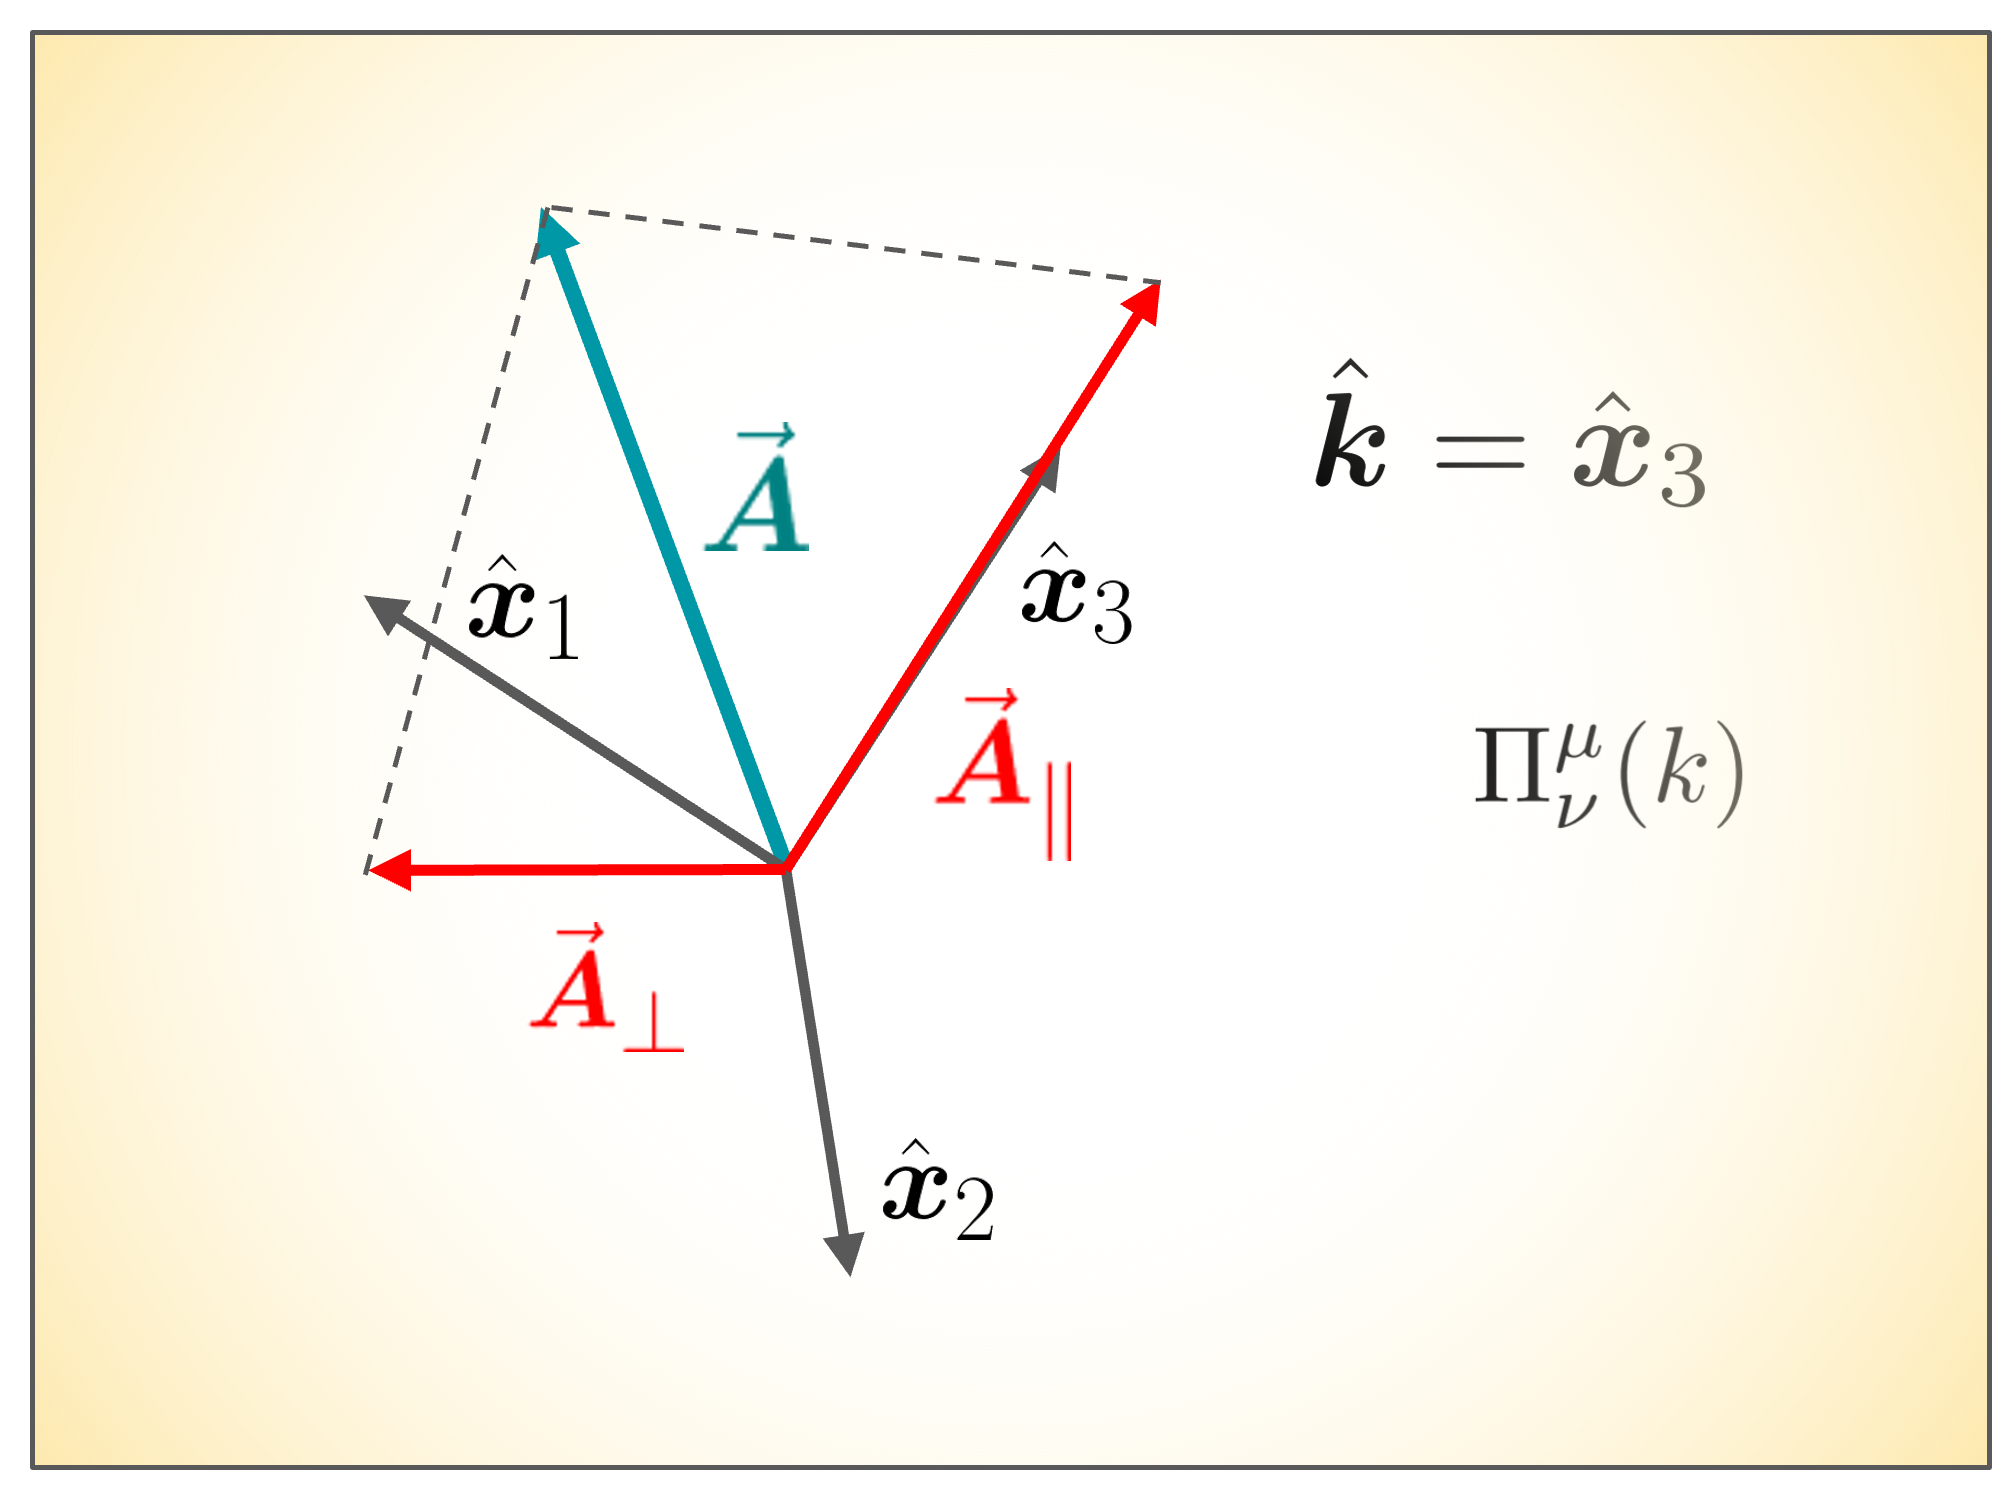
\includegraphics[width=0.55\linewidth]{plots/chap01intro/Screenshot 2024-03-14 124133.png}
    \caption{Vector potential is projected onto $\boldsymbol{\hat{k}} = \boldsymbol{\hat{x_3}} =\boldsymbol{\hat{z}}$.}
    \label{fig:project}
\end{figure}
with analogous definitions for the current, $\widetilde{j}_{\parallel}$ and $\widetilde{j}_{\perp}$. Note that the Lorentz gauge condition $\partial_\mu A^\mu = 0$ implies
\begin{equation}\label{eq:apar}
\widetilde{A}_\parallel = \frac{\omega}{ |\boldsymbol{k}|}\widetilde{\phi}\, ,
\end{equation} 
with $\phi=A^0$. The induced charge is calculated using the projected polarization tensor \req{eq:poltenmat}:
\begin{equation}
    \widetilde{\rho}_\text{ind}(\omega,\boldsymbol{k})  = \Pi^0_\nu \widetilde{A}^\nu = -\frac{|\boldsymbol{k}|^2}{\omega^2} \Pi_{\parallel}\widetilde{\phi} +  \frac{|\boldsymbol{k}|}{\omega}\Pi_{\parallel} \widetilde{A}_{\parallel}\,.
\end{equation}
For the Lorentz gauge condition \req{eq:apar}, one finds
\begin{equation}\label{eq:indch}
    \widetilde{\rho}_\text{ind}(\omega,\boldsymbol{k})  = \Pi_{\parallel}\widetilde{\phi} \left(1 -\frac{|\boldsymbol{k}|^2}{\omega^2}\right)\,.
\end{equation}
The longitudinal current is,
\begin{equation}\label{eq:indjpar}
\widetilde{j}_{\parallel\text{ind}}(\omega,\boldsymbol{k})  =  \Pi^z_\nu \widetilde{A}^\nu  = \Pi_{\parallel}  \frac{\omega}{|\boldsymbol{k}|}\widetilde{\phi}\left(1-\frac{|\boldsymbol{k}|^2}{\omega^2} \right)\,,
\end{equation}
as expected from current conservation $\partial^\mu j_\mu(x) =0$.
The induced transverse current is
\begin{equation}\label{eq:indjperp}
   \boldsymbol{j}_{\perp\text{ind}}(\omega,\boldsymbol{k})  =  \Pi_{\perp} \widetilde{A}_\perp\,.
\end{equation}
Solving for the potential on both sides of \req{eq:Amu} with the help of \reqs{eq:indch}{eq:indjperp} gives the self-consistent solutions \cite{Grayson:2022asf}
\begin{align}\label{eq:phi}
&\widetilde{\phi}(\omega,\boldsymbol{k}) = \frac{\widetilde{\rho}_\text{ext}(\omega,\boldsymbol{k})}{\varepsilon_0(\boldsymbol{k}^2-\omega^2) \left(\Pi_{\parallel}/( \omega^2\varepsilon_0)+1\right) }\,, \\\label{eq:aperp}
&\widetilde{\boldsymbol{A}}_\perp(\omega,\boldsymbol{k}) = \frac{\mu_0 \widetilde{\boldsymbol{j}}_{\perp \text{ext}}(\omega,\boldsymbol{k})}{\boldsymbol{k}^2 - \omega^2 - \mu_0 \Pi_{\perp}}\,.
\end{align}
The gauge condition \req{eq:apar} gives the self-consistent potential $\widetilde{A}_\parallel$. These self-consistent potentials determine the electric and magnetic fields via the usual relations
\begin{equation}\label{eq:ftfields}
\widetilde{\boldsymbol{B}}(\omega,\boldsymbol{k}) = i\boldsymbol{k} \times \widetilde{\boldsymbol{A}}_\perp\,, \quad \widetilde{\boldsymbol{E}}(\omega,\boldsymbol{k}) = -i \boldsymbol{k} \widetilde{\phi} + i \omega \widetilde{\boldsymbol{A}}\,.
\end{equation}
To obtain the electromagnetic fields in position space, one must Fourier transform \reqs{eq:phi}{eq:aperp}. If done analytically, this usually requires finding the poles in the denominator of these expressions, which equates to finding the poles of the thermal photon propagator. These poles represent propagating modes in the plasma. Modes will often be located at complex values in the $\omega, \mathbf{k}$ plane leading to finite lifetimes and spatial dispersion. 

\paragraph{Small back-reaction limit.} Here, we briefly mention an alternative to the self-consistent fields, which comes from assuming that the back reaction of the plasma due to the external fields is small compared to the external field. In this case, one can use the external field in the linear response equation instead of the total field
\begin{equation}\label{eq:pert}
    \widetilde{j}_{\mathrm{ind}}^{\mu}(k) = {\Pi^{\mu}}_{\nu}(k) \widetilde{A}_\text{ext}^{\nu}(k)\,.
\end{equation}
Inserting this into \req{eq:Amu} successively to find a series expansion yields the same expression as expanding \reqs{eq:phi}{eq:aperp} in the polarization functions
\begin{align}\label{eq:phipert}
&\widetilde{\phi}(\omega,\boldsymbol{k}) = \sum_{n=0}^\infty\frac{\widetilde{\rho}_\text{ext}(\omega,\boldsymbol{k})}{\varepsilon_0(\boldsymbol{k}^2-\omega^2)}\left(-\frac{\Pi_{\parallel}}{ \omega^2\varepsilon_0}\right)^n\,, \\\label{eq:aperppert}
&\widetilde{\boldsymbol{A}}_\perp(\omega,\boldsymbol{k}) = \sum_{n=0}^\infty\frac{\mu_0 \widetilde{\boldsymbol{j}}_{\perp \text{ext}}(\omega,\boldsymbol{k})}{(\boldsymbol{k}^2 - \omega^2)^{n+1}}(\mu_0 \Pi_{\perp})^{n}\,.
\end{align}
The first term $n=0$ is the vacuum field, and higher-order terms describe the back reaction of the induced current on the external field. Notably, the series expansion of \req{eq:aperp} does not accurately represent the late-time magnetic field in QGP during heavy ion collisions. This is because the infinite series of \reqs{eq:phi}{eq:aperp} must be performed to capture the pole structure of the field. 

Electromagnetic fields in a polarizable medium are often described using the electric displacement field $\mathbf{D}$, the magnetic fields $\mathbf{H}$, the polarization $\mathbf{P}$, and the magnetization $\mathbf{M}$. This formulation is only useful when the field or the medium's response is static or time-dependent. When introducing spatial and temporal dispersion, these definitions are no longer unique \cite{melrose2008quantum}. For instance, if the magnetization depends on space and time $\mathbf{M}(t,x)$ the time dependence of the magnetic field generated will lead to electric fields through Faraday's Law leading to ambiguity since the displacement field no longer depends on just polarization field $\mathbf{P}$.


\subsection{General properties of EM fields in a plasma}
In the case of an infinite homogeneous plasma, its properties are completely described by two independent polarization functions $\Pi_\parallel(k)$ and $\Pi_\perp(k)$. In the framework presented here, the properties of these scalar functions are imparted on the electromagnetic fields via the poles in the Fourier transform of the propagators in \reqs{eq:phi}{eq:aperp}. After contour integration, one effectively gets a sum of different electromagnetic fields at each pole, the amplitude of which depends on the residue of the pole, and a spacetime dependence, leading to growth attenuation or propagation depending on the pole's location. An example of this process in done in \cite{Grayson:2022asf}, where we Fourier transform the magnetic field in the center of heavy ion collisions. 

\paragraph{Dispersion relation:}
We can find the poles of the propagator or equivalently the zeros of the dispersion relation by inverting Maxwell's equations
\begin{equation}
    -ik_{\mu}\widetilde{F}^{\mu \nu} = \mu_0( \widetilde{j}_{\mathrm{ind}}^{\nu}+\widetilde{j}_{\mathrm{ext}}^{\nu})\,.
\end{equation}
Including the induced current on the left-hand side of the equation and writing the expression in terms of $A^{\mu}$ one finds,
\begin{equation}
    (k^2g^{\mu \nu} - k^{\mu} k^{\nu} + \mu_0\Pi^{\mu \nu})\widetilde{A}_{\nu} = - \mu_0\widetilde{j}_{\mathrm{ext}}^{\nu} \,.
\end{equation}
The propagator $D^\mu_\nu(k)$ is obtained by inverting the previous equation
\begin{equation}
    \widetilde{A}_{\nu}(k) = -D^{\mu}_{\nu}(k) \,\widetilde{j}_{\mathrm{ext}}^{\nu}(k) \,.
\end{equation}
The poles of $D^\mu_\nu(k)$ are given by the dispersion equation~\cite{melrose2008quantum}:
\begin{equation}\label{eq:disp}
 \frac{1}{(k\cdot u)^2}\left[(k\cdot u)^2+ \mu_0\Pi_\parallel(k)\right]\left[k^2 + \mu_0 \Pi_\perp(k)\right]^2=0 \,.
\end{equation}
The transverse mode has duplicate solutions as it describes modes in a plane perpendicular to $\boldsymbol{k}$.

The dispersion \req{eq:disp} can be solved for numerous choices of variables describing the modes such as frequency, phase velocity, or wavevector. We chose to solve for the modes of the plasma in terms of frequency $\omega_m (\mathbf{k})$ which can be thought of as a quasi-particle $m$ with energy $\omega$ and momentum $\mathbf{k}$ analogous to the usual momentum energy relation 
\begin{equation}
    E^2 = \boldsymbol{p}^2 +m^2\, ,
\end{equation}
with $c=1$. This is not always the best choice for simplifying the solutions of \req{eq:disp}, but these modes are often the easiest to interpret. A study of the modes for the general polarization tensor is not the most informative process unless one is looking for general behavior which can be found in most plasma physics textbooks. Usually, in looking at these modes $\omega_m(\mathbf{k})$, one must first assume the external field's shape or some flow distribution in the plasma by specifying the equilibrium momentum distribution to yield interesting effects in the modes such as plasma instabilities.

When the plasma is perturbed in time in a way that doesn't depend on space, such as for a plane wave, one can take $k \to 0$ for both the transverse and longitudinal roots of the dispersion relation which reduces the frequency of plasma oscillations \cite{Formanek:2021blc,Grayson:2022asf}
\begin{equation}\label{plasmafreq}
    \omega_{\pm} = -\frac{i\kappa}{2} \pm \sqrt{\omega_p^2 - \frac{\kappa}{4}^2}\,,
\end{equation}
the plasma frequency $\omega_p$ is explicitly given in the ultrarelativistic and non-relativistic limits, respectively, by \cite{Formanek:2021blc}:
\begin{equation}
\omega_p^2 = \frac{1}{3} m_D^2 \quad (\mathrm{UR})\,, \qquad \omega_p^2 = m_L^2 \quad (\mathrm{NR}) \,,
\end{equation}
with
\begin{equation}
    m_D^2 = \frac{e^2 T}{3}\,.
\end{equation}
The Debye screening mass $m_D$ describes the strength of polarization in the plasma. The plasma frequency $\omega_p$ is the characteristic response frequency of the plasma. For an external field which is an oscillatory wave of the form $E=E_0e^{-i\omega t}$, one would find that the response is weakly-damped or over-damped depending on the size of $\kappa$ according to \req{eq:plasmafreq}. Waves are weakly damped for $\kappa \ll \omega_p$, and since the square root is imaginary for $\kappa > 2\omega_p$, waves become over-damped. These general statements are subject to the spacetime dependence of the external perturbation. For instance, if a particle moves through the plasma at a constant velocity, the field will not experience much damping if the velocity is much less than the speed of sound in the plasma.

In the static limit $\omega \rightarrow 0$ the zeros in the longitudinal dispersion relation take on the form
\begin{equation}
    |\mathbf{k}| = \pm  i m_D \,.
\end{equation}
Fourier transforming using the positive root in \req{eq:phi} gives the Debye-H\"uckel screening of a stationary charge within the plasma \cite{Debye:1923}
\begin{equation}
    \phi(r) = \frac{Z \alpha \hbar c \, e^{-r/\lambda_D}}{r}\,, \quad \text{with} \quad  \lambda_D = \frac{m_D}{\hbar c}\,.
\end{equation}
The Debye length $\lambda_D$ describes the size of the polarization cloud around a charge generated by the plasma.
\paragraph{Permittivity, susceptibility, and conductivity:}

In most fields of applied physics the effects of a polarizable medium on electromagnetic fields are not described by the polarization functions $\Pi_\parallel$ and $\Pi_\perp$. It is instructive to connect these quantities to more commonplace definitions such as relative permittivity $\epsilon$, susceptibility $\chi$, and conductivity $\sigma$.

The dielectric and susceptibility tensors are related to the spatial portion of the polarization tensor $\Pi^i_j$ ~\cite{Starke:2014tfa,melrose2008quantum},
\begin{equation}\label{dielten}
     \boldsymbol{K}^i_j(\omega,\boldsymbol{k}) = \boldsymbol{\varepsilon}^i_j/\varepsilon_0 = 1+\frac{\boldsymbol{\Pi}^i_j(\omega,\boldsymbol{k})}{\omega^2} = 1+\boldsymbol{\chi}^i_j(\omega,\boldsymbol{k})\,.
\end{equation}
When we project on the axis $\mu =3$, the spatial portion of the polarization tensor is
 \begin{equation}
    \boldsymbol{\Pi}^{i}_{j}(\omega,\boldsymbol{k}) = \left[
    \begin{array}{ccc}
  \Pi_{\perp} & 0 & 0 \\
  0 & \Pi_{\perp} & 0 \\
  0& 0 & \Pi_{\parallel} \\ 
\end{array}
\right]\,.
\end{equation}
It is then natural to discuss transverse and longitudinal susceptibilities,
\begin{equation}\label{eq:chi}
    \chi_\parallel(\omega,\boldsymbol{k}) =\frac{\Pi_\parallel(\omega,\boldsymbol{k})}{\omega^2}, \quad \text{and} \quad \chi_\perp(\omega,\boldsymbol{k}) = \frac{\Pi_\perp(\omega,\boldsymbol{k})}{\omega^2}\,.
\end{equation}
and their associated permeabilities $K_\parallel$ and $K_\perp$. These quantities are useful for studying the attenuation of electromagnetic fields by looking at light absorption.

The conductivity tensor is found by taking the spatial part of the linear response equation \req{eq:ohm} and expressing the vector potential in terms of the electric field $i \omega \widetilde{A^i} = \widetilde{E^i}$~\cite{Starke:2014tfa,melrose2008quantum}
\begin{align}\label{eq:sigmaperp}
    \sigma_\perp(\omega,\boldsymbol{k}) &\equiv - i \omega \chi_\perp(\omega,\boldsymbol{k}) =- i \frac{\Pi_\perp(\omega,\boldsymbol{k})}{\omega} \,,\\
    \sigma_\parallel(\omega,\boldsymbol{k}) &\equiv - i \omega \chi_\parallel(\omega,\boldsymbol{k}) =- i \frac{\Pi_\parallel(\omega,\boldsymbol{k})}{\omega} \,.
\end{align} 
The long wavelength limit $k \to 0$ the conductivity reduces to the Drude model of conductivity~\cite{Drude:1900} with $\tau = 1/\kappa$
\begin{equation}\label{eq:drude}
    \sigma_\parallel(\omega,0) = \sigma_\perp(\omega,0) = \frac{\sigma_0}{1-i \omega/\kappa} \,.
\end{equation}
with the static conductivity given by
\begin{equation}\label{eq:condstat}
   \sigma_0 = \frac{m_D^2}{3\kappa}\,.
\end{equation} 
The Drude model is equivalent to solving the Vlasov-Boltzmann equation using the Anderson-Witting collision term \req{eq:lincoll} and neglecting spatial dispersion.

These quantities are discussed in detail and plotted in \cite{Formanek:2021blc}. While these quantities are useful for communicating the physics of plasma response, the limits of these quantities must be taken carefully to retain the causal properties of the field. Specifically, tacitly expanding these quantities in either $\omega$ and $\mathbf{k}$ and then inserting them into the self-consistent potentials \reqs{eq:phi}{eq:aperp} will not necessarily generate causal solutions. Instead of carefully expanding and taking limits of these quantities to ensure analyticity, it's often easier to expand the electromagnetic fields within their Fourier transforms as is done in Appendix B of \cite{Grayson:2022asf}.

%%%%%%%%%%%%%%%%%%%%%%%%%%%%%%%%%%%%%%%%%%%%%%%%%%%%%%%%%%%%%%%%%%%%%%%%%%%%%%%%%%%%%%
\subsection{Advances in linear response: discussion and outlook}

The main result of \cite{Formanek:2021blc} is the polarization tensor \req{eq:pimunu} which is an appropriate solution for an infinite polarizable medium with damping due to collisions. Additionally, the analytic form of this tensor in phase space is found in the ultrarelativistic and non-relativistic limits. The addition of current conservation leads to a correction in the longitudinal portion of the polarization tensor compared to the one found using the Anderson-Witting collision term.

Here, we only consider electrons and positrons, neglecting the effects of spin. Our framework would be improved by incorporating spin into our kinetic description of plasmas. This could be done by taking the classical limit of the quantum kinetic transport of the Wigner function as in \cite{Hurst:2014svf}. This would be especially important in quark-gluon plasmas, where we study the magnetic field. Below, we will summarize a few areas of future work advancing the description of plasmas presented here. 

\paragraph{Energy conserving collision term:}
The polarization tensor \req{eq:pimunu} conserves current but not explicitly energy. Energy conservation can be ensured by adding a correction to the collision term similar to \req{eq:collision} but involving the second moment of $\delta f$ which is related to energy-momentum density \cite{Rocha:2021zcw}
\begin{multline}
    C = - (p\cdot u) \kappa\bigg[\delta f(x,p) -\frac{\delta n(x) }{ \eq{n} } -\eq{\Gamma_1}(x,p)\frac{\int (dq) (q\cdot u)\eq{\Gamma_1}(q) \delta f(x,q) }{\int (dq) (q\cdot u) (\eq{\Gamma_1}(q))^2 \eq{f}(q) }...\\
    -\mathcal{P}^{\mu \nu}p_\nu\frac{\int (dq) (q\cdot u)\mathcal{P}^{\mu \nu}q_\nu \delta f(x,q) }{\int (dq) (q\cdot u) \mathcal{P}^{\mu \nu}q_\nu\mathcal{P}_{\mu \beta}q^\beta \eq{f}(q) }
    \bigg]\,,
\end{multline}
where we use $q$ to distinguish momenta being integrated over and $\Gamma_1(x,p)$ is defined as
\begin{equation}
    \Gamma_1(x,p) = 1-(p\cdot u)\frac{\int (dq) (q\cdot u)f(x,q)}{\int (dq) (q\cdot u)^2f(x,q)}
    = 1-\frac{ (p\cdot u) n(x)}{T^{00}(x)}\,,
\end{equation}
and analogously
\begin{equation}
    \eq{\Gamma_1}(p) = 1-(p\cdot u)\frac{\int (dq) (q\cdot u)\eq{f}(q)}{\int (dq) (q\cdot u)^2\eq{f}(q)}
    = 1-\frac{ (p\cdot u) \eq{n}}{T_{(\text{eq})}^{00}} \,.
\end{equation}
The projector operator$\mathcal{P}^{\mu \nu}(u)$ is 
\begin{equation}
    \mathcal{P}^{\mu \nu}(u) = g^{\mu \nu} -u^\mu u^\nu\,.
\end{equation}
We show in \cite{Grayson:2022asf} that the energy-momentum violation cancels in the current for a matter-antimatter plasma. Finding the polarization tensor, including energy-momentum conservation, is the subject of future work. The addition of this term in the current is studied in relativistic hydrodynamics in \cite{Singha:2023eia}. Instead of adding these complex correction terms, it may be better to use the Fokker-Planck equation or its simplified counterpart the LBO or Doughtery collision term \cite{Dougherty1964,Francisquez:2022imd,Ong:1970evs}, which manifestly conserves energy-momentum and current, and is better suited to study electromagnetic grazing collisions. 
\paragraph{Applications to other plasmas:}
The main motivation of this work was to derive a relativistic polarization tensor that could be used to describe quark-gluon plasma and other plasmas where damping is important. In Chapter \ref{chap:QCD} we discuss the application of the ultrarelativistic limit of the polarization tensor to study the electromagnetic properties of QGP. This polarization tensor is easy to generalize to other ultrarelativistic antimatter plasmas. Since the particles are massless, increasing the number of plasma particle species merely leads to an enhancement of the Debye mass \cite{Grayson:2022asf,Kapusta:1992fm}
\begin{equation}\label{eq:Debyem}
    {m_D}^2_{(\text{EM})} = \sum_{u,d,s} q^2_f T^2 \frac{N_c}{3} \equiv C_{\text{em}}T^2\,,
\end{equation}
where $C_{\text{em}} =  2e^2/3$. We implement the non-relativistic solution to the polarization tensor to study the screening of thermonuclear reactions in BBN by electron-positron plasma. This discussion can be found in Chapter \ref{section_electron}.

If considering a plasma of particles of different masses, such as an electron-proton plasma, one needs only to find a polarization tensor for each particle species and then sum them up in the induced current \req{eq:perturbation1}.

\paragraph{Fully relativistic polarization tensor:}
One can evaluate the integrals in \req{eq:pimunu} by assuming an appropriate equilibrium distribution to find the polarization tensor. As mentioned above this is done for the ultrarelativistic and the non-relativistic limits in \cite{Formanek:2021blc}. For the full relativistic calculation, relevant for plasma where the temperature is on the order of the mass of the plasma constituents $m\approx T$, one must integrate the relativistic Fermi function. This can be done by writing it in the series representation \cite{Letessier:2002ony}
\begin{equation}
\begin{split}
     f_\mathrm{eq}(|\pmb{p}|) &= \frac{1}{e^{\sqrt{|\boldsymbol{p}|^2+ m^2}/T} + 1} \\
     &= \sum_{n=1}^{\infty} (-1)^{n+1}\left( e^{-\sqrt{|\boldsymbol{p}|^2+ m^2}/T}\right)^n\,,
    \end{split}
\end{equation}
whose integral results in an infinite sum of Bessel functions of the second kind, for instance when calculating the equilibrium density one finds
\begin{equation}
    n_\mathrm{eq}=\frac{1}{\pi^2}T^3\sum_{n=1}^{\infty}g^2\frac{ (-1)^{n+1} K_2\left(\frac{n}{m}\right)}{ n}\,.
\end{equation}
The modified Bessel functions of the second kind $K_2(x)$ with the $(-1)^{n+1}$ alternate between exponential growth and decay as $n$ increases. This complicates the calculation of the polarization tensor since the angular integrals and momentum integrals no longer factor out in $R^\mu_\nu$, $Q^\mu$, $H_\nu$, and $Q$. Such a calculation would be necessary to investigate the thermal mass of quarks in QGP.

\paragraph{Linear response in strong fields:}
We are interested to see if we can generalize this framework to strong fields where the Coulomb interaction energy is close to the thermal energy
\begin{equation}
    \frac{ qA(x)\cdot U}{T}\approx 1\,.
\end{equation}
We feel it should be possible to derive the electromagnetic field in plasma for small perturbations away from the strong field equilibrium 
\begin{equation}
    f(x,p) = f_\text{eq}(x,p) + \delta f (x,p)\,,
\end{equation}
where in the Boltzmann limit the strong field equilibrium distribution is \cite{Hakim:2011bk,Hakim:1967prd}
\begin{equation}
     f_\text{eq}(x,p) = \exp \left(-u_{\mu}[p^{\mu}+q A^{\mu}(x)]/T\right)\,.
\end{equation}
Of course, this assumes the strong field equilibrium solution is stable under electromagnetic perturbations. As of the writing of this document, it seems that the assumption of linear response is incompatible with strong fields, indicating that the plasma response in the strong fields cannot be described by a polarization tensor, as outlined in this chapter. A resolution to this topic requires further investigation.


\paragraph{Mixed-species collision term:}
We also hope to generalize this framework to involve a Vlasov-Boltzmann equation system that represents each plasma species with a different collision term. In matrix form, this system of Boltzmann equations for an electron-positron plasma would look like
\begin{equation}\label{eq:vectoreq}
-i (p \cdot k) \left[\begin{matrix}
\wt{\delta f}_- \\ \wt{\delta f}_+ 
\end{matrix}\right] + (u \cdot \wt{F} \cdot p)\left[\begin{matrix}
q_-\peq{f}_- \\ q_+\peq{f}_+
\end{matrix}\right] = (p \cdot u) \left[\begin{matrix}
\kappa_{--} & \kappa_{-+}\\
\kappa_{-+} & \kappa_{++}
\end{matrix}\right]\left[\begin{matrix}
\wt{C}(f_-) \\ \wt{C}(f_+)
\end{matrix} \right]\,.
\end{equation}
One can then use a separate collision rate to represent the collisions between different species. The issue here is that the BGK collision term approximates collisions in the plasma as a medium effect so this system of equations is trivial since it does not allow momentum transfer between distributions of different species. In future work, we would like to propose a new collision term that allows momentum transfer between species but is still simpler than the microscopic collision term \req{eq:collisionMicro}.





%============================================================================
% \subsection{Polarization tensor}

% In order to evaluate the integrals $Q^\mu$, $H_\nu$, $Q$ and $R^\mu_\nu$ we choose to orient the vector $\pmb{k}$ along the $z$-axis
% \begin{equation}
% k^\mu = (\omega,0,0,k)\,.
% \end{equation}
% With this choice the gauge condition imposed on the polarization tensor (\ref{eq:transversal2}) becomes
% \begin{equation}\label{eq:gaugeincomponents}
% \Pi^0_z = -\frac{\omega}{k}\Pi^0_0, \quad \Pi^z_z = - \frac{\omega}{k}\Pi^z_0\,.
% \end{equation}
% We choose to perform the calculations in the rest frame of the medium $u^\mu = (1,0,0,0)$ and in two limits where, either the mass can be neglected (ultrarelativistic limit), or where the plasma particle move slowly compared with the speed of light (nonrelativistic limit).


% %==================================================================================
% \subsection{Ultrarelativistic limit}

% In this limit we neglect the mass of the plasma particles as compared to their momentum. With this assumption the non-zero components of the polarization tensor are (see Appendix \ref{sec:ultrarel} for details):
% \begin{align}
% \Pi^0_0 &= - m_D^2 L \left( 1+ \frac{i\kappa\Lambda}{2k-i\kappa\Lambda} \right)\,,\\
% \Pi^0_z &=m_D^2 \frac{\omega}{k}L \left( 1+ \frac{i\kappa\Lambda}{2k-i\kappa\Lambda} \right)\,,\\
% \Pi^z_0 &= -m_D^2\frac{\omega}{k}L\left(1 + \frac{i\kappa \Lambda}{2k - i\kappa \Lambda}\right)\,,\\
% \Pi^z_z &= m_D^2\frac{\omega^2}{k^2}L\left(1 + \frac{i\kappa \Lambda}{2k - i\kappa \Lambda}\right)\,,\\
% \Pi^x_x &= \Pi^y_y = \frac{m_D^2\omega}{4k}\left( \frac{\omega'^2}{k^2}\Lambda - \Lambda - \frac{2\omega'}{k}\right)\,.
% \end{align}
% The quantities $\omega'$, $\Lambda$, and $L$ are defined as
% \begin{align}\label{eq:definitions}
% \omega' \equiv \omega + i\kappa, \quad \Lambda \equiv \ln \frac{\omega' + k}{\omega'-k}, \quad L \equiv 1-\frac{\omega'}{2k}\Lambda\,,
% \end{align}
% and the Debye screening mass $m_D^2$ is given by integral (\ref{eq:mD}):
% \begin{equation}\label{eq:debye}
% m_D^2 \equiv \frac{q^2T^3}{3}\,.
% \end{equation}

% %==================================================================
% \subsection{Nonrelativistic limit}

% In this limit we assume that the velocity of the plasma particles is much smaller than the speed of llight, i.~e., we work in the low temperature limit $T \ll m$. We also assume that $|\pmb{p}|k/m\omega' \ll 1$ in order to be able to perform the expansion in the momentum integrals. We refer to Appendix \ref{sec:nonrel} for the derivation of the results. The non-zero components of the polarization tensor are: 
% \begin{align}
% \Pi^0_0 &= m_L^2 \frac{k^2}{\omega'^2} \frac{1}{1-\frac{i\kappa}{\omega'}\left(1+\frac{T k^2}{m\omega'^2} \right)}\,,\\
% \Pi^0_z &= -m_L^2 \frac{\omega k}{\omega'^2} \frac{1}{1-\frac{i\kappa}{\omega'}\left(1+\frac{T k^2}{m\omega'^2} \right)}\,,\\	
% \Pi^z_0 &= m_L^2 \frac{\omega k}{\omega'^2} \frac{1}{1-\frac{i\kappa}{\omega'}\left(1+\frac{T k^2}{m\omega'^2} \right)}\,,\\	
% \Pi^z_z &= -m_L^2 \frac{\omega^2}{\omega'^2} \frac{1}{1-\frac{i\kappa}{\omega'}\left(1+\frac{T k^2}{m\omega'^2} \right)}\,,\\
% \Pi^x_x &= \Pi^y_y = -m_L^2 \frac{\omega}{\omega'}\,.
% \end{align}
% Here we have introduced the mass scale $m_L^2$ through the integral (\ref{eq:mL})
% \begin{equation}
% m_L^2 \equiv q^2 \left(\frac{2mT}{\pi}\right)^{3/2}\frac{e^{-m/T}}{2m}\,.
% \end{equation}	
% We shall see in Section \ref{sec:disp} below that $m_L$ is the nonrelativistic plasma frequency.

% %======================================================================
% \subsection{Current conservation in components}

% The current conservation relation (\ref{eq:currentconserv}) reads in explicit component notation:
% \begin{equation}
% 0 = k_0 \Pi^0_0 \widetilde{A}^0 + k_0 \Pi^0_z \widetilde{A}^z + k_z \Pi^z_0 \widetilde{A}^0 + k_z \Pi^z_z \widetilde{A}^z\,.
% \end{equation}
% To do show that the right-hand side vanishes as required, we invoke the Lorentz gauge condition $k \cdot \widetilde{A}=0$ which allows us to express $\widetilde{A}^z$ in terms of $\widetilde{A}^z$:
% \begin{equation}
% \widetilde{A}^z = \frac{\omega}{k}\widetilde{A}^0\,.
% \end{equation}
% The current conservation condition now becomes a constraint on the polarization tensor alone:
% \begin{equation}\label{eq:currentcomputation}
% 0 = \Pi^0_0 + \frac{\omega}{k}\Pi^0_z - \frac{k}{\omega}\Pi^z_0 - \Pi^z_z\,. 
% \end{equation}
% If we invoke the gauge invariance constraint (\ref{eq:gaugeincomponents}) we can simplify
% \begin{equation}
% 0 = \left(1-\frac{\omega^2}{k^2} \right)\left(\Pi^0_0 - \Pi^z_0 \frac{k}{\omega}\right)\,.
% \end{equation}
% The current conservation condition is now reduced to the constraint
% \begin{equation}\label{eq:currentconservcomp}
% \Pi^z_0 = \frac{\omega}{k}\Pi^0_0\,,
% \end{equation}
% which is obviously satisfied in both limits. In conclusion, the polarization tensor $\Pi^\mu_\nu$ conserves the electric current and ensures its gauge invariance. With both covariant indices $\Pi_{\mu\nu}$ is even symmetric.

% %===================================================================
% \subsection{Collective Plasma Behavior}

% The equivalent dielectric and susceptibility tensors, through  which  one  can  study  collective  plasma  effects, are defined through the spatial portion of the polarization tensor $\Pi^i_j$ as in~\cite{Starke:2014tfa,melrose2008quantum},
% \begin{equation}\label{dielten}
%      K^i_j(\omega,k) = \varepsilon^i_j/\varepsilon_0 = 1+\frac{\Pi^i_j(\omega,k)}{\omega^2} = 1+\chi^i_j(\omega,k)
% \end{equation}
% For an isotropic plasma the spatial part can be written in terms of two independent response functions, one ($\Pi_T$) transverse to $\mathbf{k}$, the other ($\Pi_L$) parallel to $\mathbf{k}$. These are immediately recognizable in the spatial components of $\Pi^{\mu}_{\nu}$, evaluated in the rest frame, given that $\mathbf{k}$ was chosen to be in the $\hat{z}$ direction~\cite{melrose2008quantum}. The longitudinal and transverse response functions are given by
% \begin{equation}\label{eq:piLT}
%     \Pi_L =\Pi^z_z = - \frac{\omega^2}{k^2}\Pi^0_0, \quad \Pi_T =\Pi^x_x=\Pi^y_y \,.
% \end{equation}
% Both prescriptions for $\Pi_L$ are equivalent because of current conservation. They arise from solving the Maxwell equations in medium for either $A_0$ or $A_\parallel$. Reference frame independent definitions of $\Pi_L$ and $\Pi_T$ can be given with the help of manifestly Lorentz invariant projection operators~\cite{melrose2008quantum}.

% %===================================================================
% \subsection{Susceptibilities}

% \begin{figure}[H]
% \centering
% 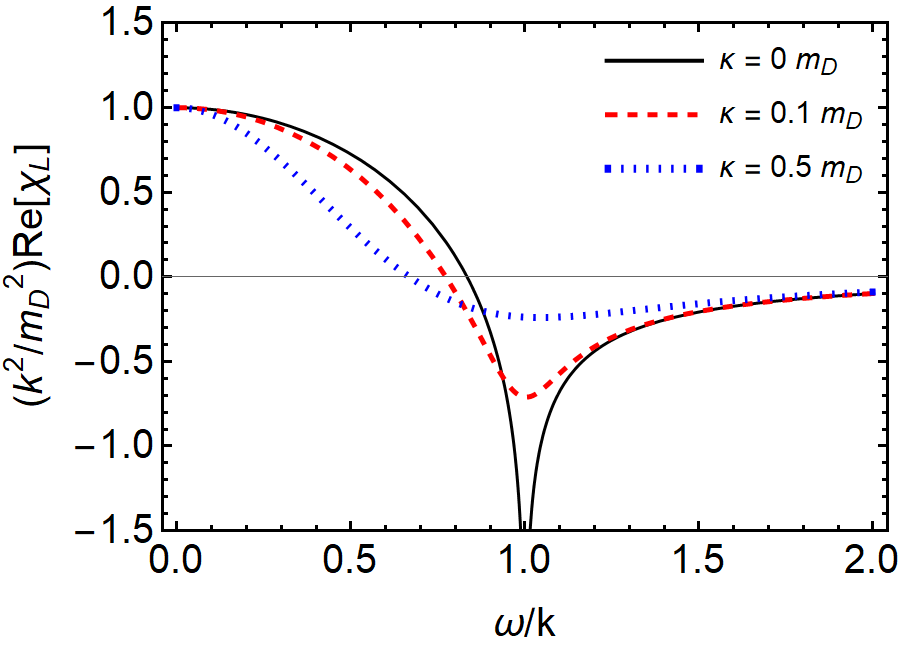
\includegraphics[width=0.95\linewidth]{plots/chap01intro/chil2dRe.png}
% \caption{The real part of the longitudinal susceptibility is plotted as a function of phase velocity $\omega/k$ for various values of the relaxation rate $\kappa$. The curve for $\kappa=0$ matches the electric susceptibility in~\cite{Weldon:1982aq}. The addition of the collision term smoothens the frequency dependence.}
% \label{fig:Re_chi_L}
% \end{figure}

% The susceptibilities describes the frequency and wavelength dependent response of the plasma to an external field. One can define the transverse and longitudinal susceptibilities through equation (\ref{dielten}) using the transverse and longitudinal response functions,
% \begin{equation}\label{eq:chi}
%     \chi_L =\frac{\Pi_L}{\omega^2}, \quad \chi_T = \frac{\Pi_T}{\omega^2}
% \end{equation}
% The real and imaginary parts of these susceptibilities are shown in Figs.~\ref{fig:Re_chi_L}--\ref{fig:chi_T3d}.
 
% \begin{figure}[H]
% \centering
% 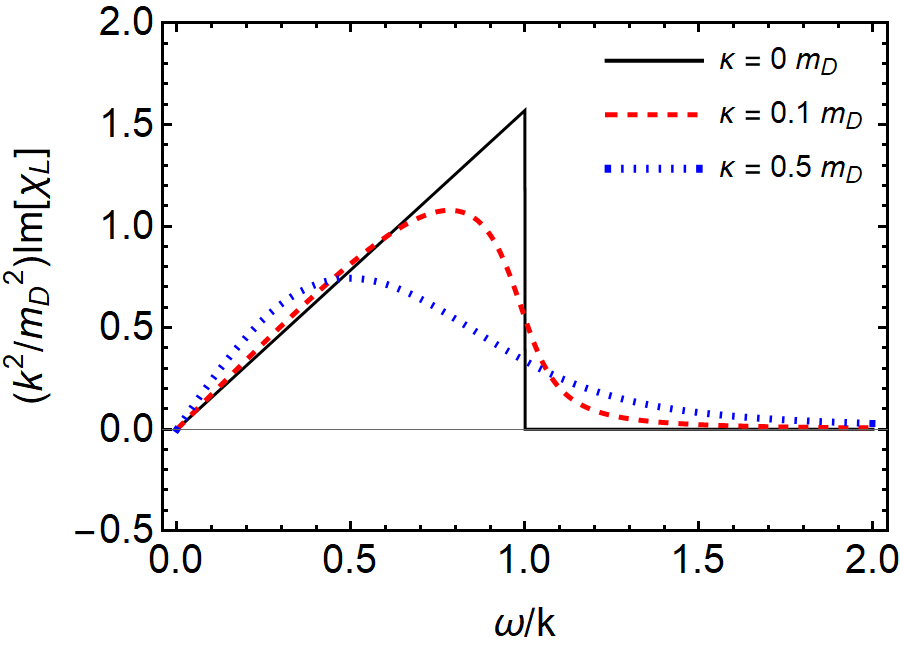
\includegraphics[width=0.95\linewidth]{plots/chap01intro/chil2dIm.png}
% \caption{The imaginary part of the longitudinal susceptibility is plotted as a function of phase velocity $\omega/k$ for various values of relaxation rate. The discontinuity of ${\rm Im}[\chi_L]$ at $\omega/k = 1$ is smoothened out for $\kappa > 0$.}
% \label{fig:Im_chi_L}
% \end{figure}

% The solid (black) line in Fig.~\ref{fig:Re_chi_L} for $\kappa=0$ reproduces the result shown in Fig.~1 of Ref.~\cite{Weldon:1982aq}. The dashed (red) and dotted (blue) lines show how the real part longitudinal susceptibility is modified for non-zero values of the collision rate ($\kappa/m_D = 0.1, 0.5$). Figure \ref{fig:Im_chi_L} shows the imaginary part of the longitudinal susceptibility as a function of $\omega/k$. One sees how the Landau damping, which in the absence of collisions ($\kappa = 0$) is constrained to the space-like momentum domain, extends into the time-like domain for $\kappa > 0$. 

% Figures~\ref{fig:chi_L3d}~and~\ref{fig:chi_T3d}~show three-dimensional plots of the real and imaginary part of $\chi_L(\omega,k)$ and $\chi_T(\omega,k)$ for $\kappa/m_D = 0.1$, respectively. The normal modes are clearly visible as features along the diagonal in the $\omega-k$ plane.
% We can expand the susceptibilities in the optical limit, $k \ll m_D$. In this limit, the longitudinal and transverse susceptibilities are given by
% \begin{equation}\label{chi_l_opt}
%    \chi_L(\omega,k) =-\frac{\omega_p^2}{\omega(\omega+i\kappa)} - \frac{\omega_p^2}{\omega^2} \frac{ ( 9 \omega+5i\kappa )}{15(\omega+ i \kappa )^3} k^2 + O\left(k^4\right) \,,
% \end{equation}
% \begin{equation}
%    \chi_T(\omega,k) = -\frac{\omega_p^2}{\omega(\omega+i\kappa)}-\frac{\omega_p^2 k^2}{5 \omega (\omega +i \kappa )^3} + O\left(k^4\right) \,,
% \end{equation}
% where $\omega_p^2 = m_D^2/3$ is the plasma frequency. Here we can clearly see that to leading order the two susceptibilities are the same as it must be for an isotropic medium. Solving the dispersion relations for the $k$ independent term gives the plasma frequency, this is done in (\ref{sec:disp}). 

% We can also expand the susceptibilities in the limit $k\gg m_D$ where one finds:
% \begin{equation}
%      \chi_L(\omega,k) = \frac{m_D^2}{k^2}-\frac{ i \pi  \omega  m_D^2}{2 k^3}+O\left(\frac{1}{k^4}\right)
% \end{equation}
% \begin{equation}
%     \chi_T(\omega,k) = -\frac{ i \pi m_D^2}{4 k \omega }-\frac{ m_D^2 (\omega +i \kappa )}{k^2 \omega }
%     +\frac{ i \pi m_D^2 (\omega +i \kappa )^2}{4 k^3 \omega }+O\left(\frac{1}{k^4}\right)
% \end{equation}
% The frequency independent term in the longitudinal susceptibility describes the phenomenon of static Debye screening, with the inverse Debye mass $1/m_D$ defining the screening length. 



% \begin{figure}[H]
% \centering
% 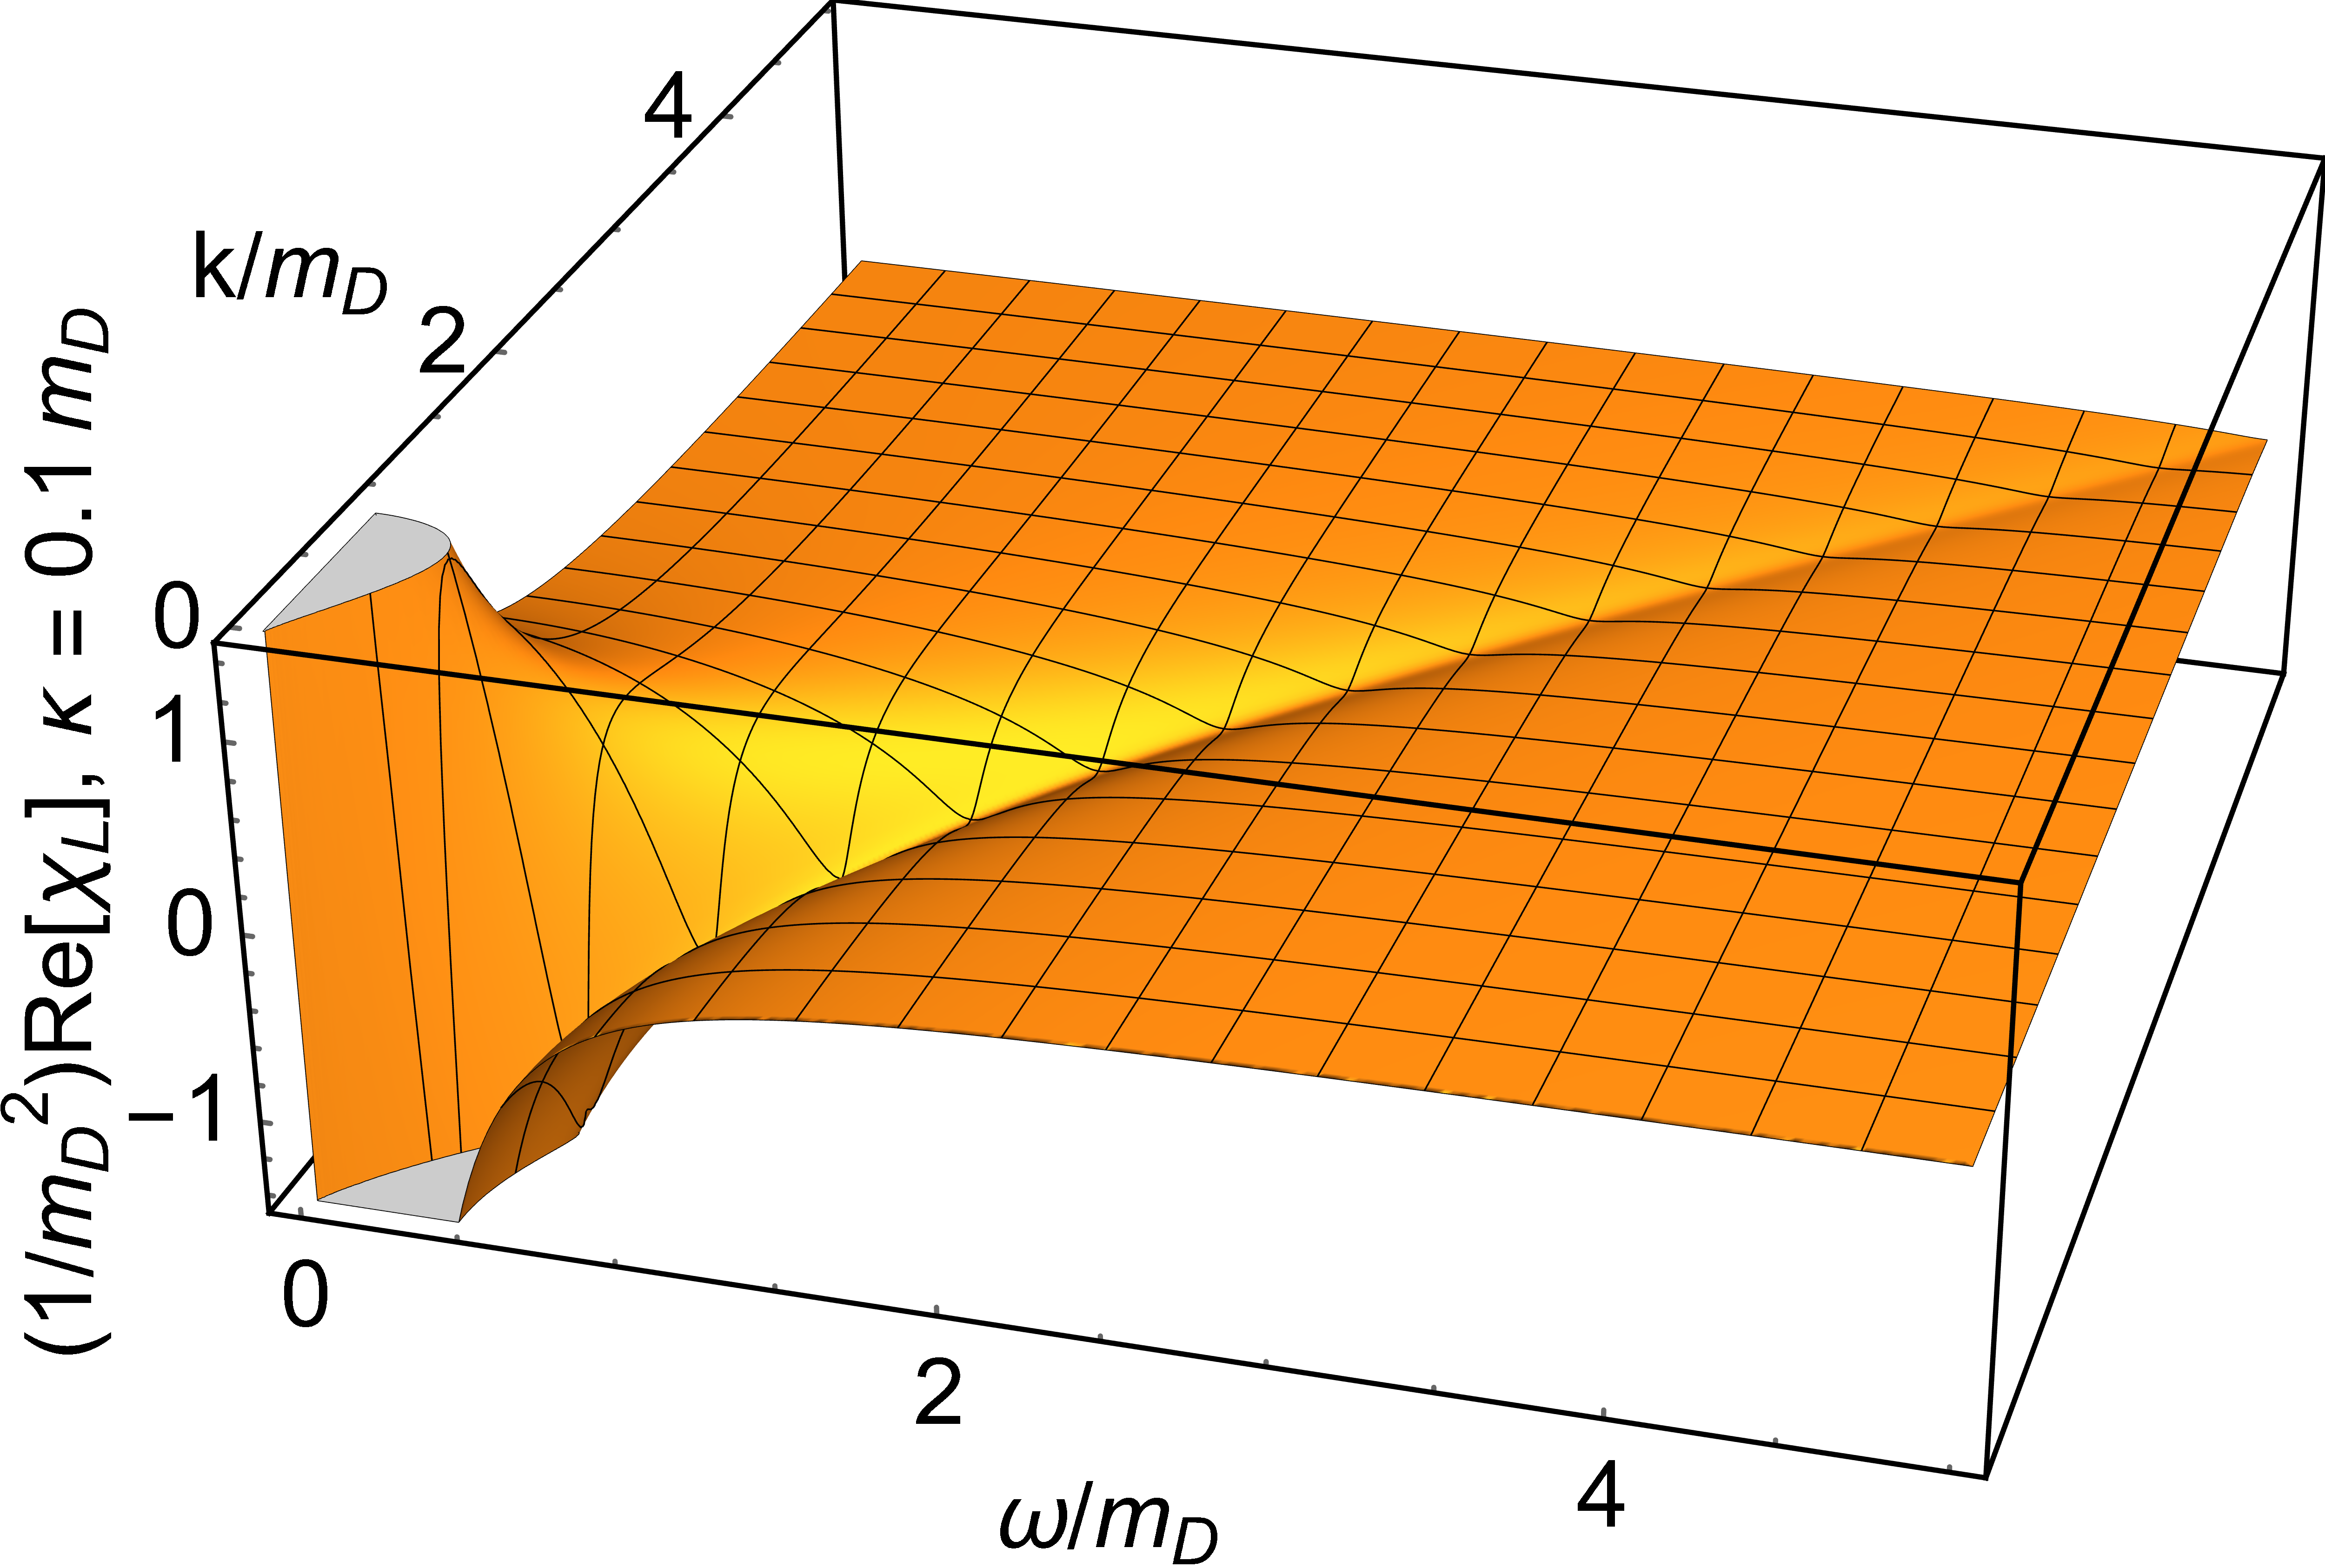
\includegraphics[width=0.45\linewidth]{plots/chap01intro/chi3dReL1.png}
% \hspace{0.05\linewidth}
% 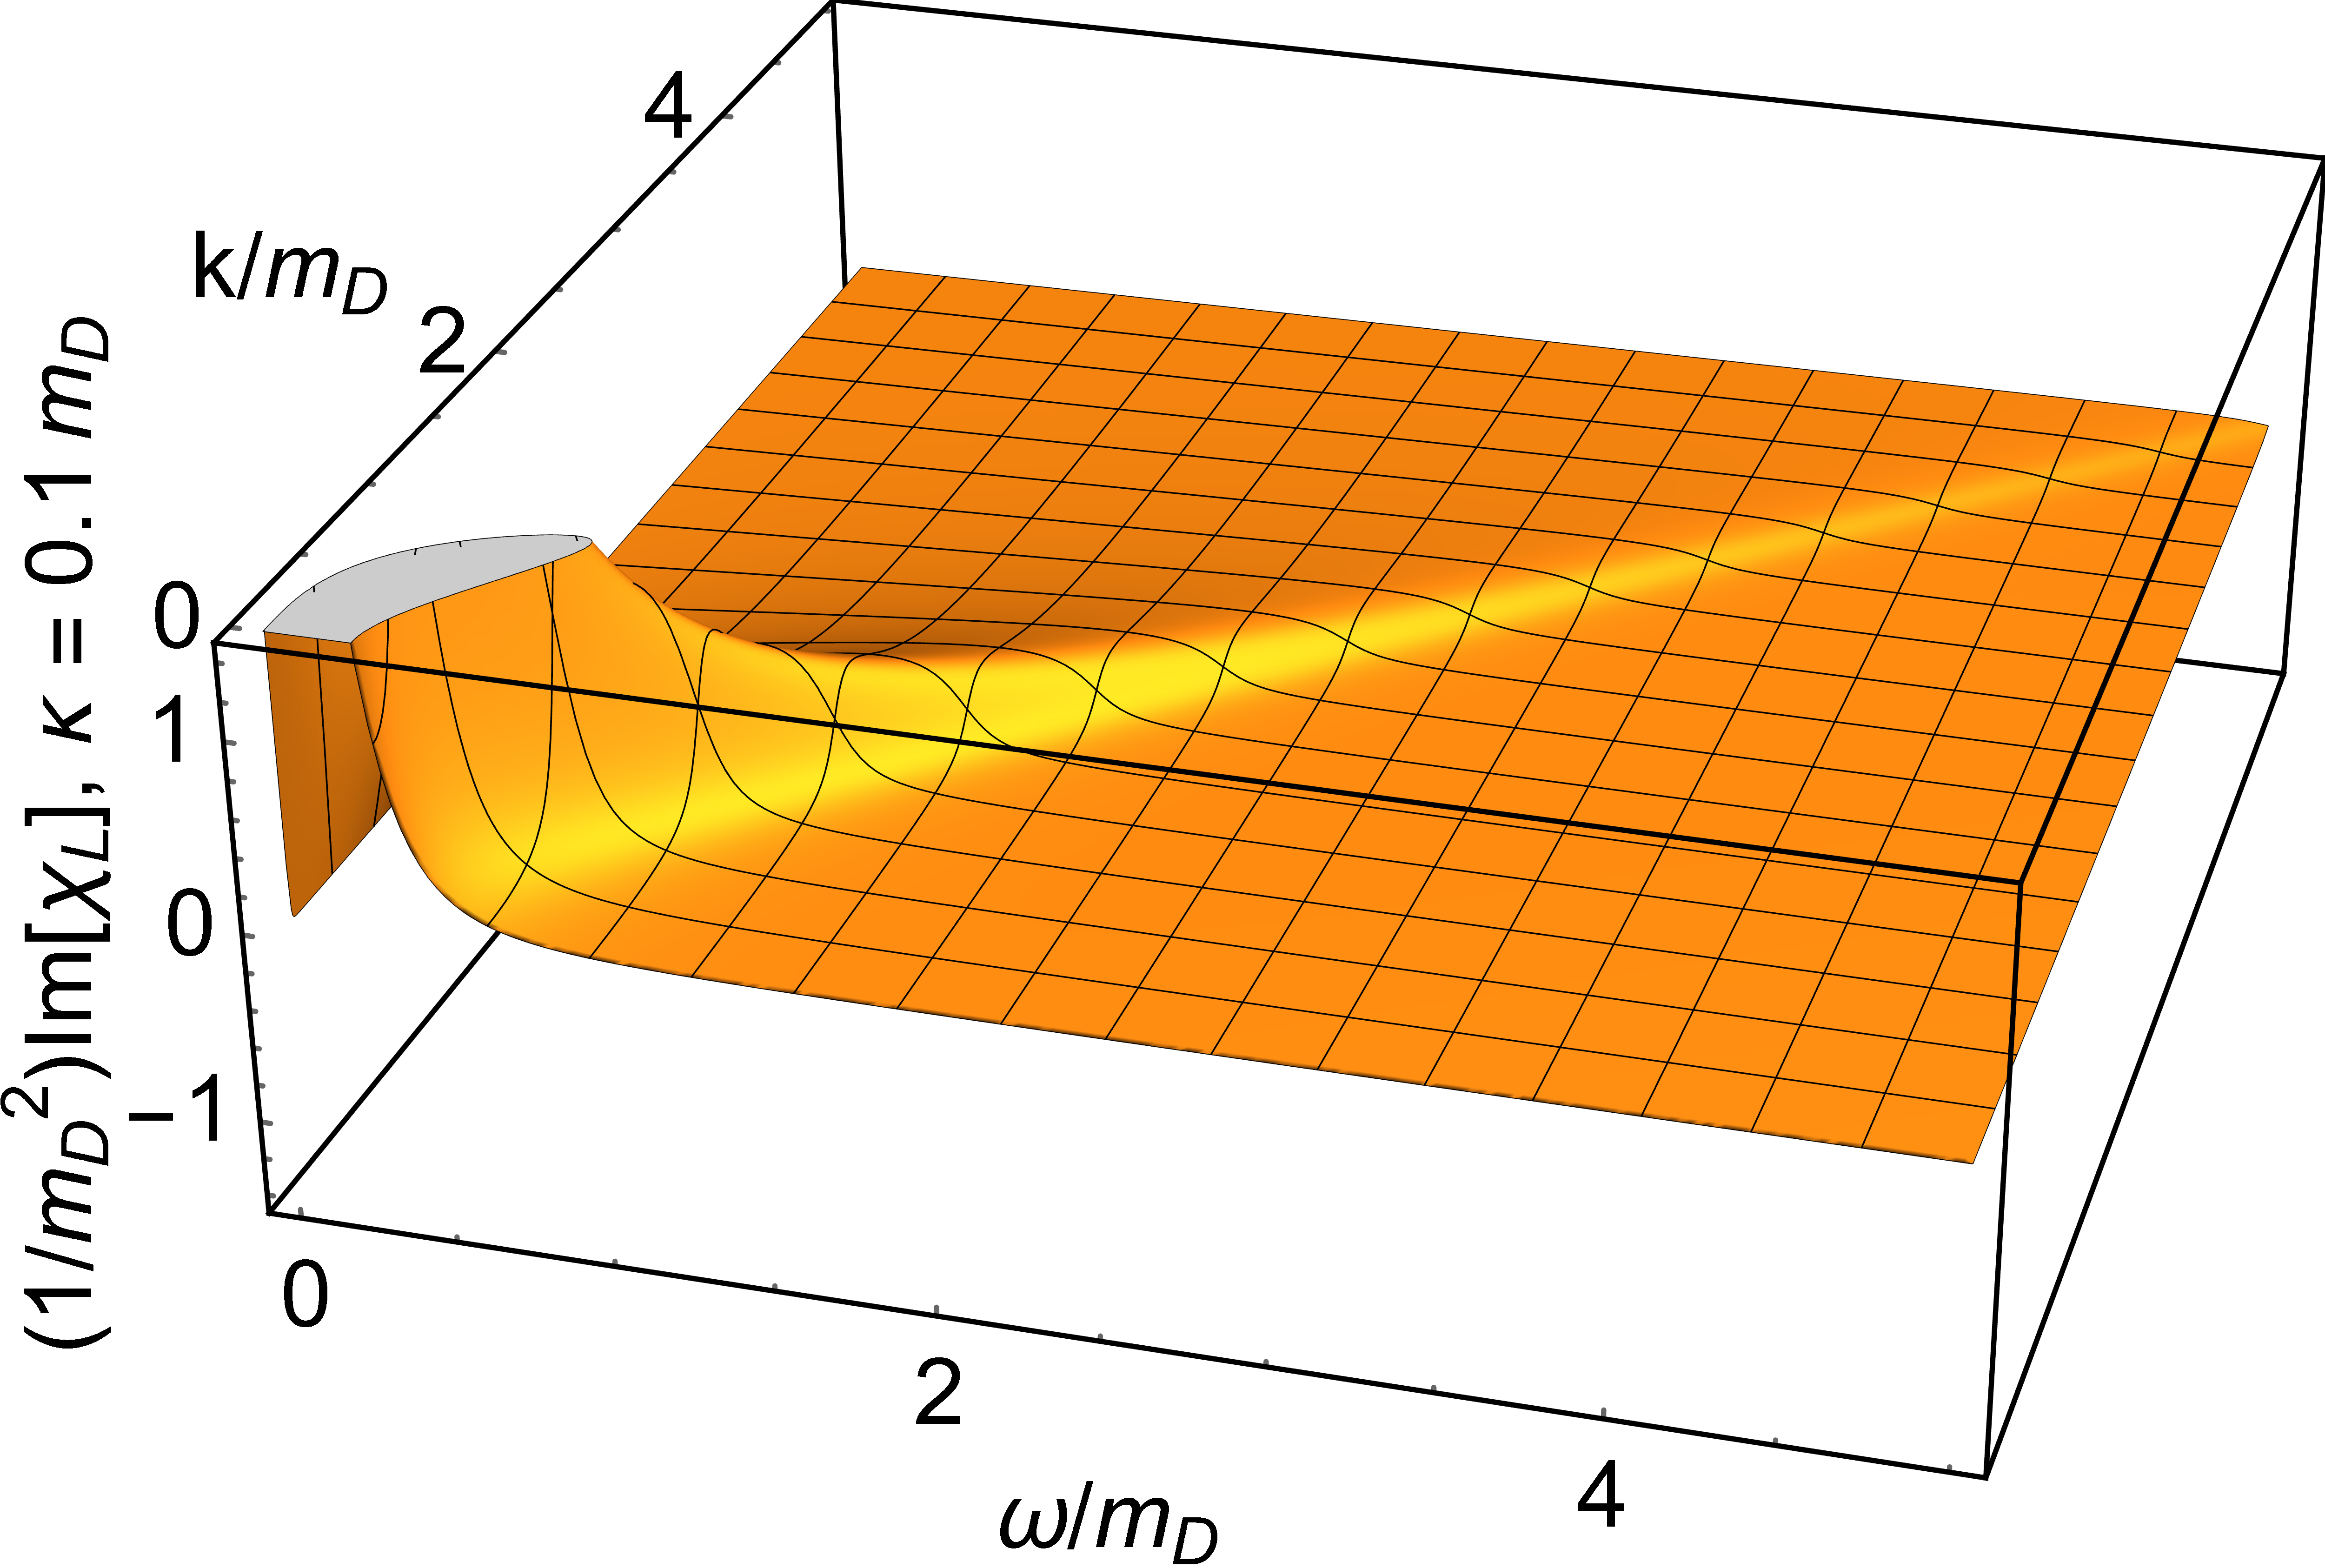
\includegraphics[width=0.45\linewidth]{plots/chap01intro/chi3dImL1.png}
% \caption{Longitudinal susceptibility $\chi_L(\omega, k)$ in units of $m_D^2$ for $\kappa = 0.1\,m_D$. Left panel: real part of $\chi_L(\omega,k)$; right panel: imaginary part of $\chi_L(\omega,k)$.}
% \label{fig:chi_L3d}
% \end{figure}

% \begin{figure}[H]
% \centering
% 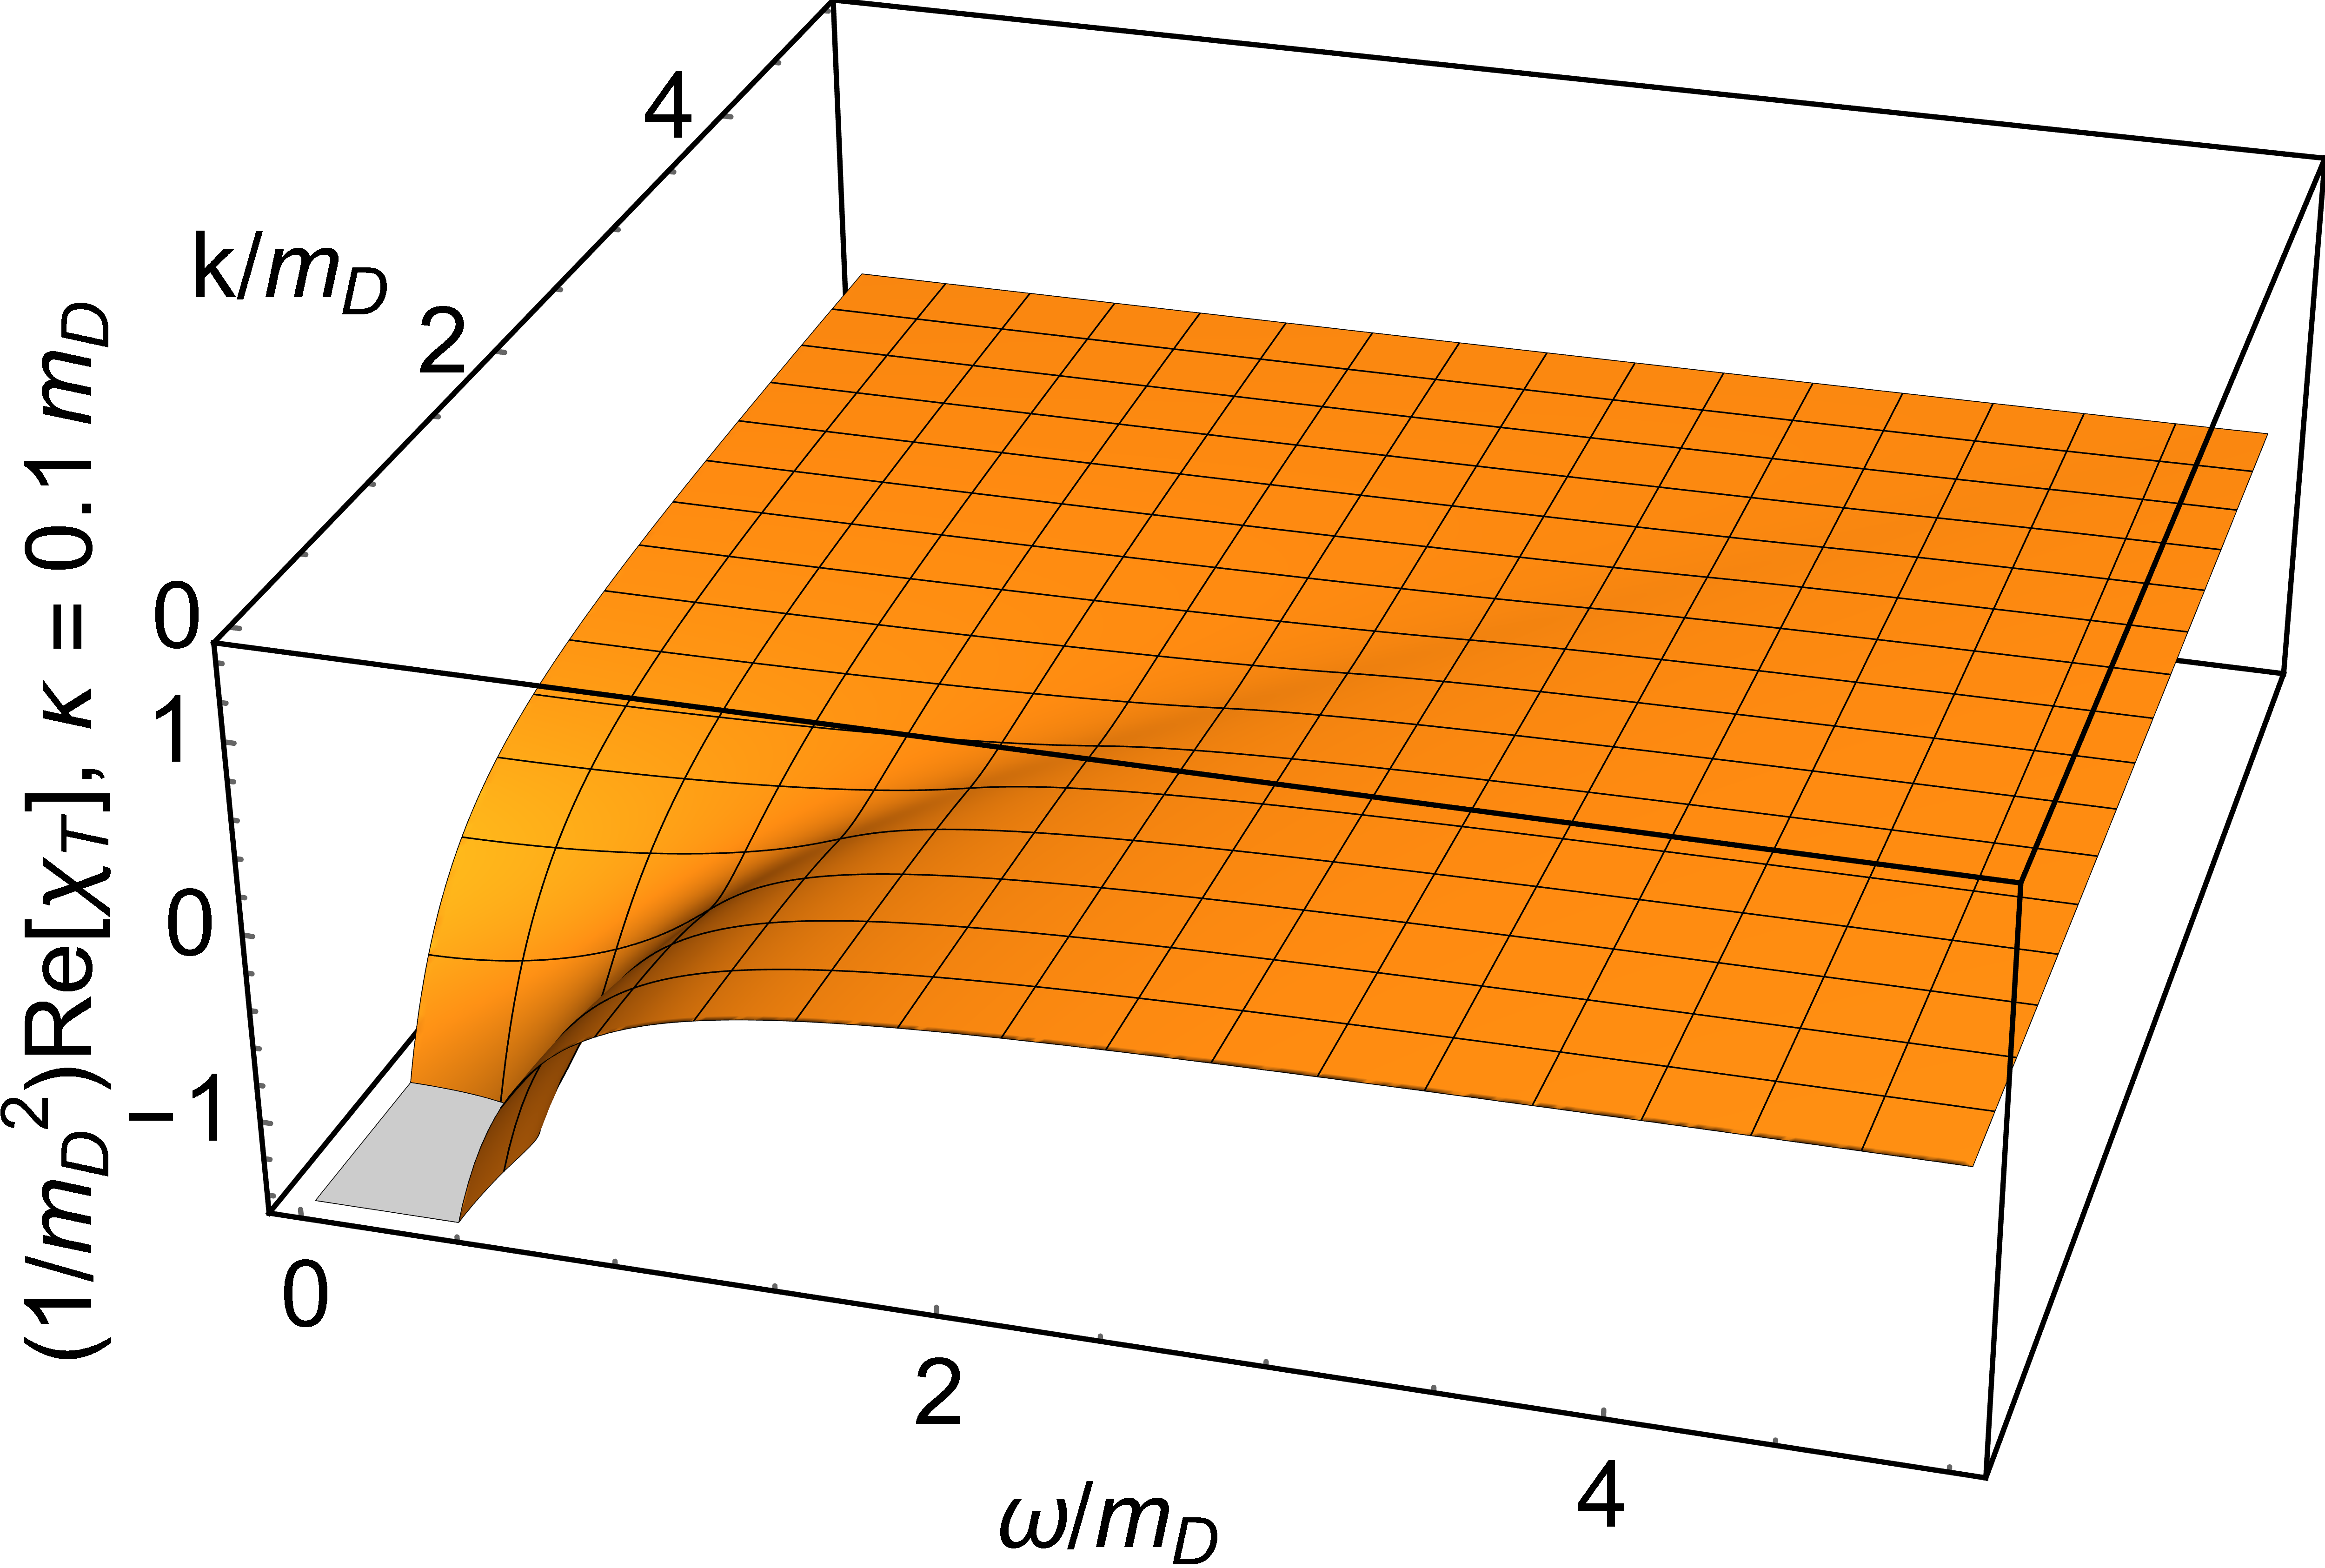
\includegraphics[width=0.45\linewidth]{plots/chap01intro/chi3dReT1.png}
% \hspace{0.05\linewidth}
% 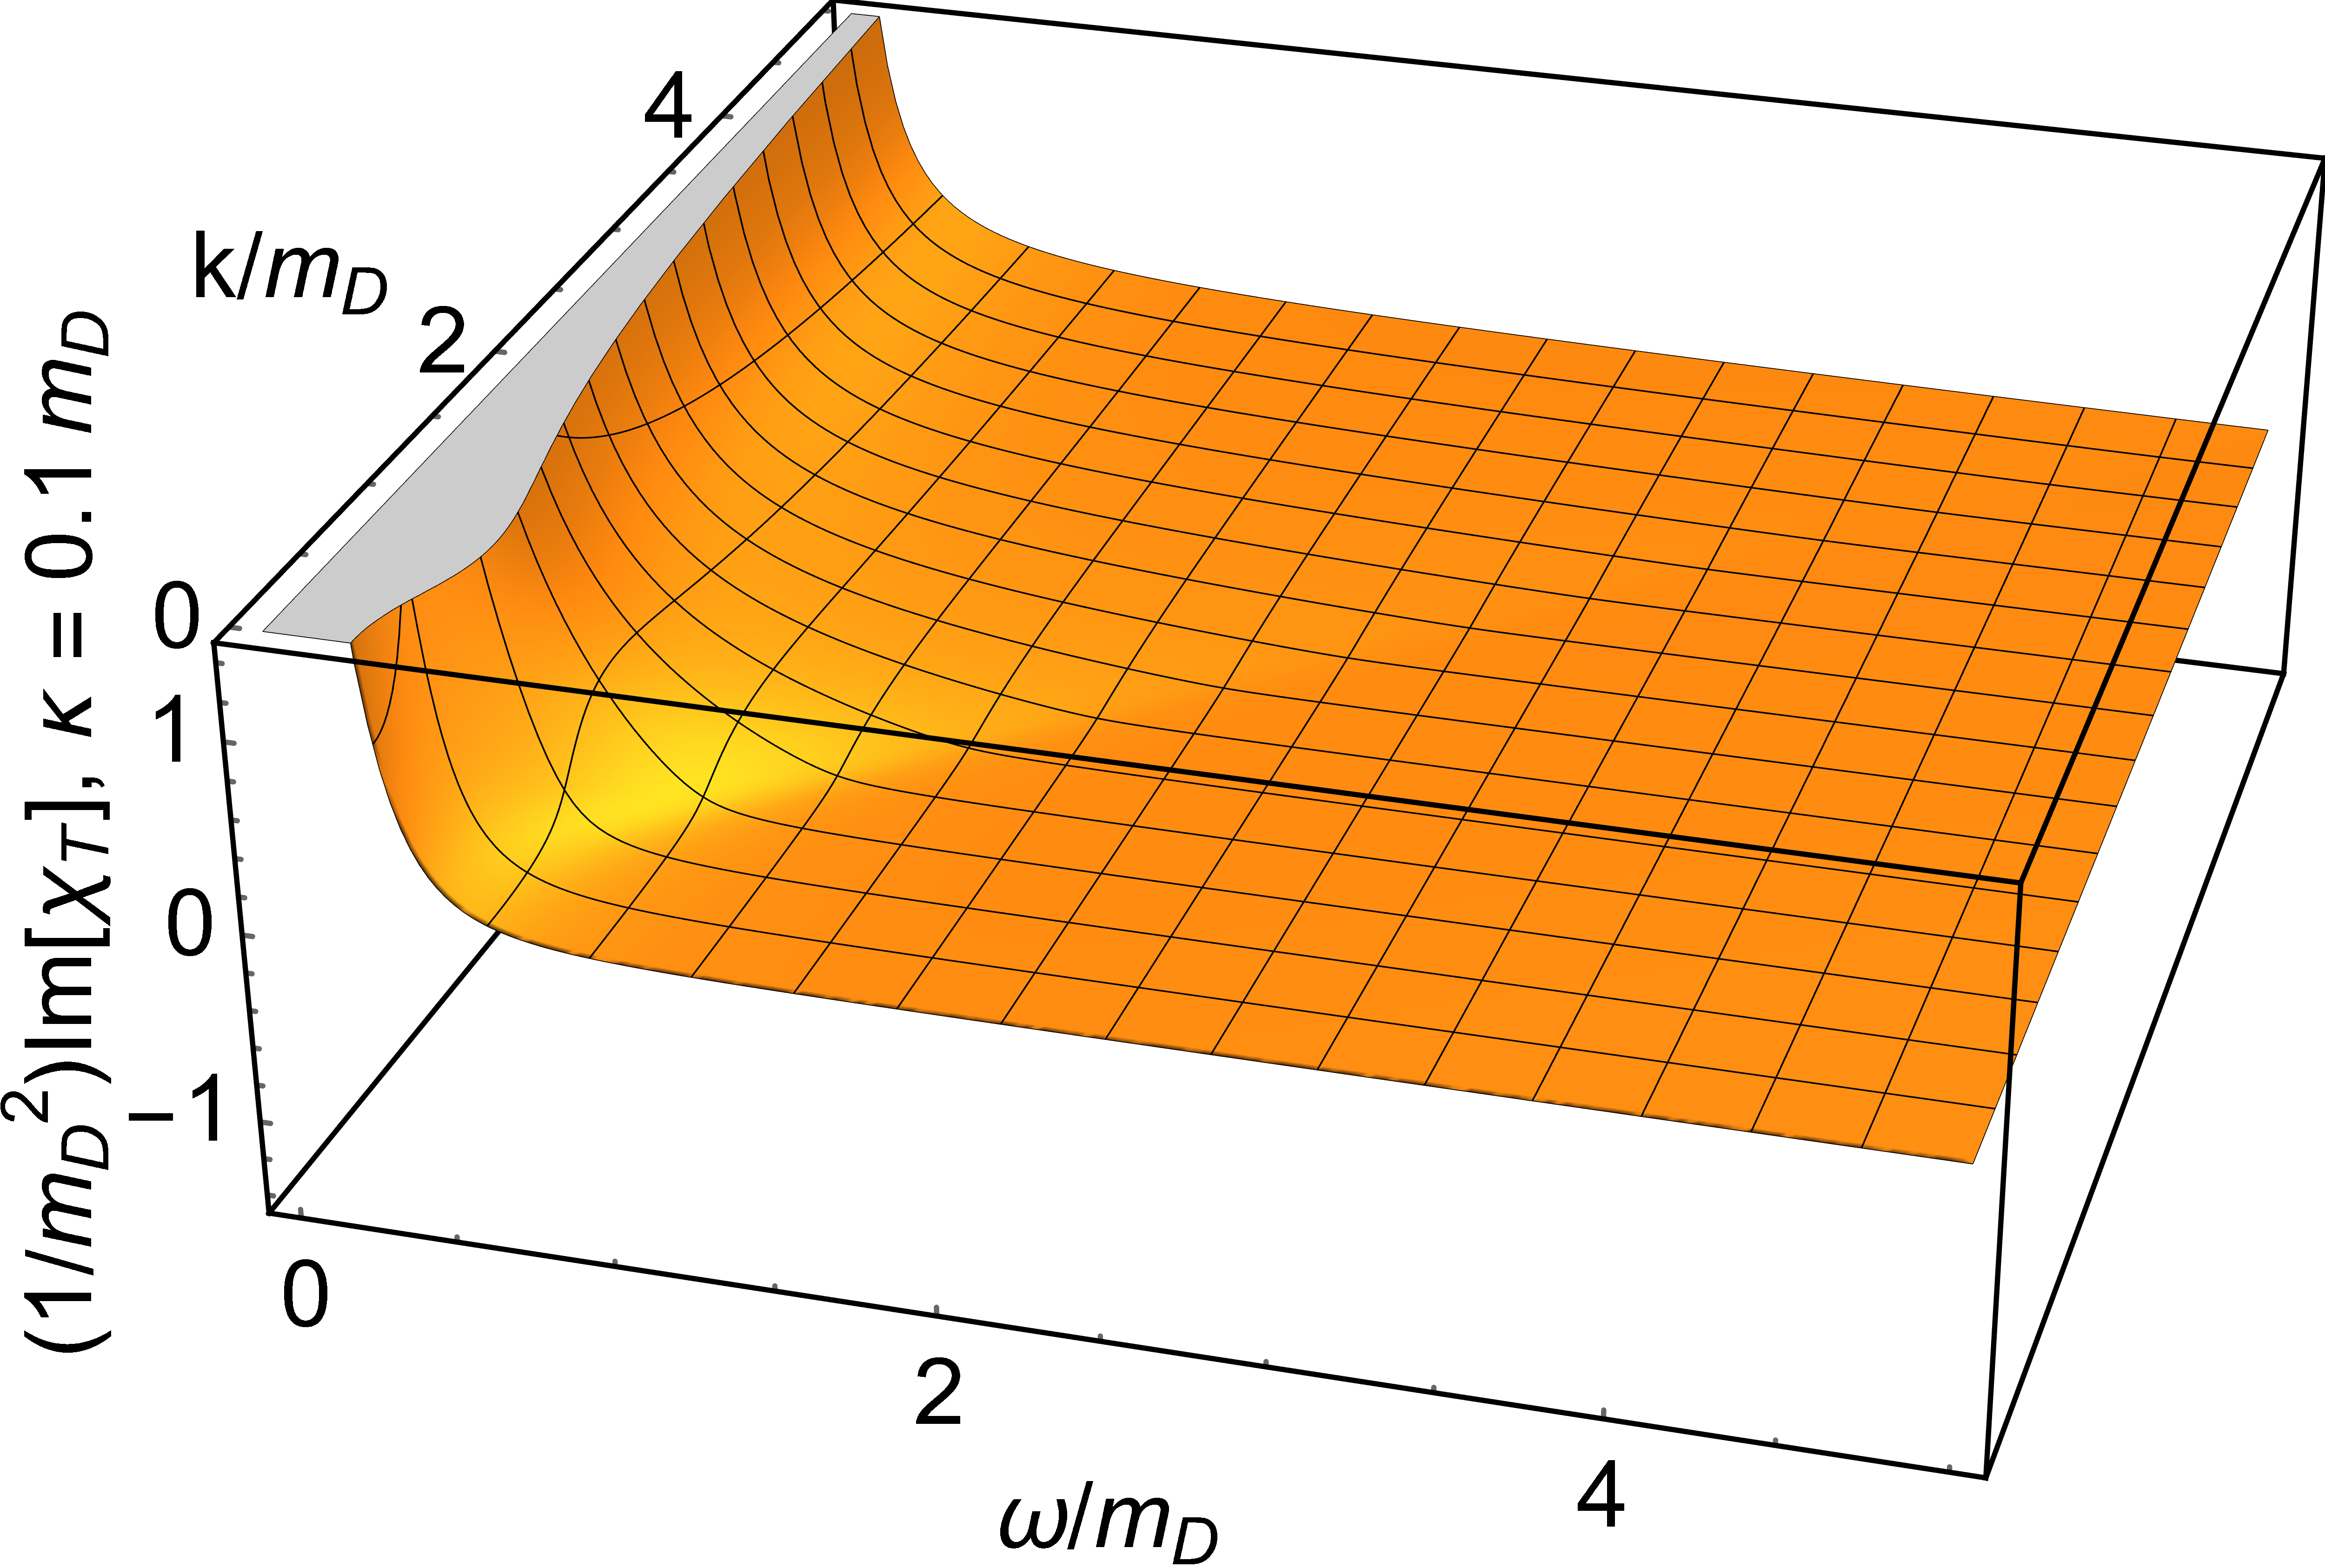
\includegraphics[width=0.45\linewidth]{plots/chap01intro/chi3dImT1.png}
% \caption{Transverse susceptibility $\chi_T(\omega, k)$ in units of $m_D^2$ for $\kappa = 0.1\,m_D$. Left panel: real part of $\chi_T(\omega,k)$; right panel: imaginary part of $\chi_T(\omega,k)$. }
% \label{fig:chi_T3d}
% \end{figure}


% We now compare our results for the BGK collision term with those obtained for the simple Anderson-Witting (AW) collision model (\ref{eq:lincoll}) which does not contain the current conserving BGK modification. This is of interest as such results appear frequently in literature. In the ultrarelativistic limit, the polarization tensor with the AW collision term is given by the tensor components $R^\mu_\nu$ from equations (\ref{eq:r00}-\ref{eq:rzz}) in Appendix \ref{sec:ultrarel}. Because $R^\mu_\nu$ alone does not satisfy the current conservation condition (\ref{eq:currentconservcomp}) there are two different possible definitions of longitudinal susceptibility $\chi_L$ constructed from either $R^z_z$ component (\ref{eq:rzz}) or the $R^0_0$ component (\ref{eq:r00}).

% To avoid confusion, we continue to call the susceptibility constructed from the $R^z_z$ component of the polarization tensor the longitudinal susceptibility $\chi_L$ and the susceptibility constructed from the $R^0_0$ component of the polarization tensor the charge susceptibility $\chi_0$. Of course, when the collision term satisfies current conservation, $\chi_0 = \chi_L$, as it is indeed the case for the BGK modified collision term (\ref{eq:boltzmanncov}). Because the current conservation is violated for $R^\mu_\nu$ the two definitions of $\Pi_L$ (\ref{eq:piLT}) do not agree with each other. In other words the solution of Maxwell equations for the scalar potential or the longitudinal component of the vector potential are no longer related as they would be when $\partial_\mu j^\mu = 0$.  

% In Figs.~\ref{fig:RechiLcomp} and \ref{fig:ImchiLcomp} we compare the real and imaginary components of the longitudinal and charge susceptibility in the BKG and AW collision models for $\kappa = 0.5 m_D$. For the BGK model there is only a single curve (the solid lines); there are two different curves for the unmodified AW model: The dashed lines show the charge susceptibility $\chi_0$; the dotted lines show the longitudinal susceptibility $\chi_L$. The fact that the two lines differ, especially in the region $\omega < k$, is a direct consequence of current conservation violation of the AW model. Our results (solid curves) are clearly different from either of the AW curves.

% We note in passing that the $\chi_L$ of the AW model, as defined by the $R^z_z$ component of the polarization tensor, is the same as we would get for the Blaizot-Iancu \cite{Blaizot:2001nr} form of the polarization tensor 
% \begin{equation}
% \Pi^\mu_\nu(k) = m_D^2 \left(-\delta^{\mu0}\delta_{\nu0} + \omega \int \frac{d\Omega}{4\pi}\frac{v^\mu v_\nu}{v \cdot k + i \kappa} \right)
% \end{equation}
% by simply substituting a nonzero value $\kappa$. However, note that this version suffers from the limitation that it is not manifestly Lorentz covariant because the 4-velocity of the medium $u^\mu$ is not explicitly introduced (compare with the covariant expression for $R^\mu_\nu$ (\ref{eq:Rmunu}) and its evaluation in Appendix \ref{sec:ultrarel}).

% \begin{figure}
% 	\centering
% 	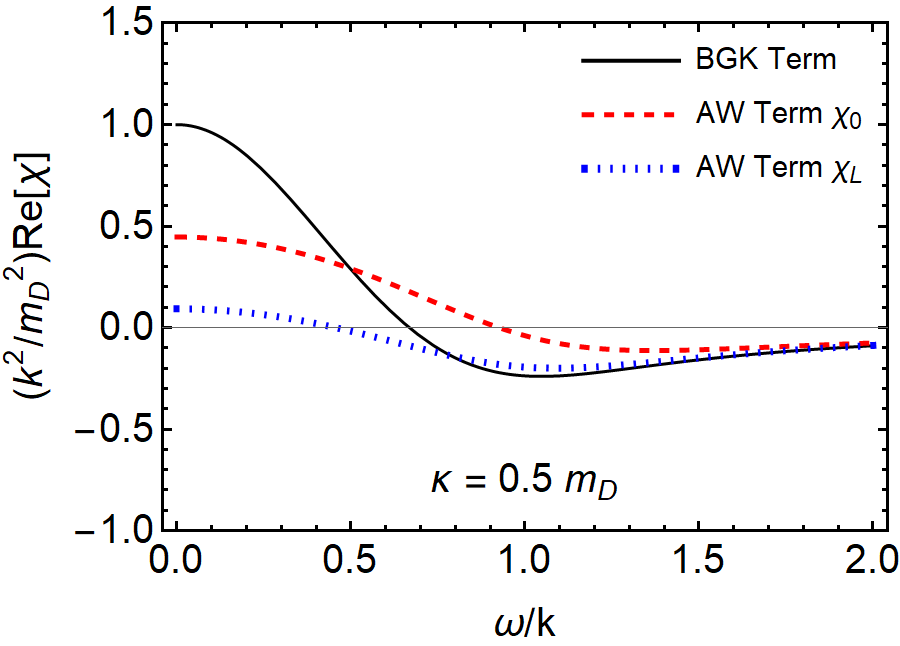
\includegraphics[width=0.95\linewidth]{plots/chap01intro/chil2Recomp.png} 
% 	\caption{Real part of $\chi_L$ as a function of $\omega/k$ for $\kappa = 0.5 m_D$. We compare the BGK collision model considered in this paper and Anderson-Witting (AW) model given by the collision term (\ref{eq:lincoll}) with both definitions of $\Pi_L$ (\ref{eq:piLT}).}	
% 	\label{fig:RechiLcomp}
% \end{figure}

% \begin{figure}
% 	\centering
% 	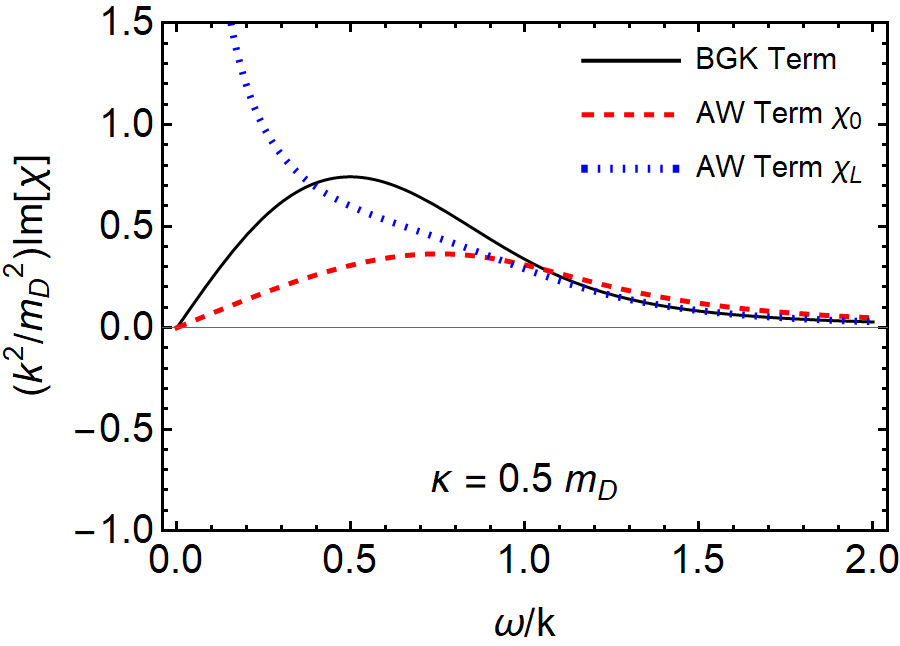
\includegraphics[width=0.95\linewidth]{plots/chap01intro/chil2Imcomp.png}
% 	\caption{Imaginary part of $\chi_L$ as a function of $\omega/k$ for $\kappa = 0.5 m_D$. We compare the BGK collision model considered in this paper and Anderson-Witting (AW) model given by the collision term (\ref{eq:lincoll}) with both definitions of $\Pi_L$ (\ref{eq:piLT}).}
% 	\label{fig:ImchiLcomp}
% \end{figure}


% %===================================================================
% \subsection{Conductivity}
% \begin{figure}
% 	\centering
% 	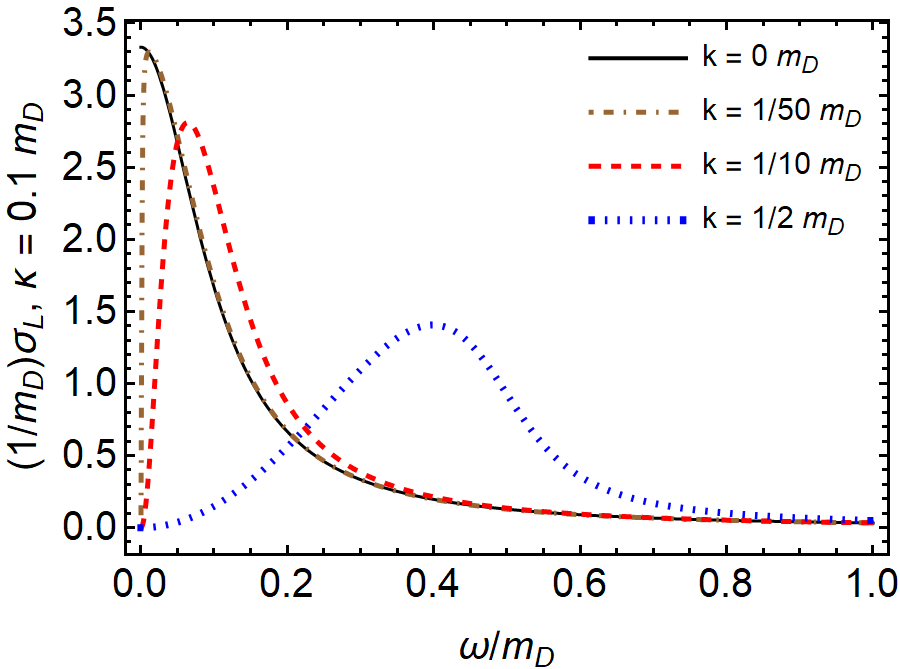
\includegraphics[width=0.95\linewidth]{plots/chap01intro/condlRe.png} 
% 	\caption{Real part of $\sigma_L$ for different values of $k$.}	
% 	\label{fig:sigma_L}
% \end{figure}

% \begin{figure}
% 	\centering
% 	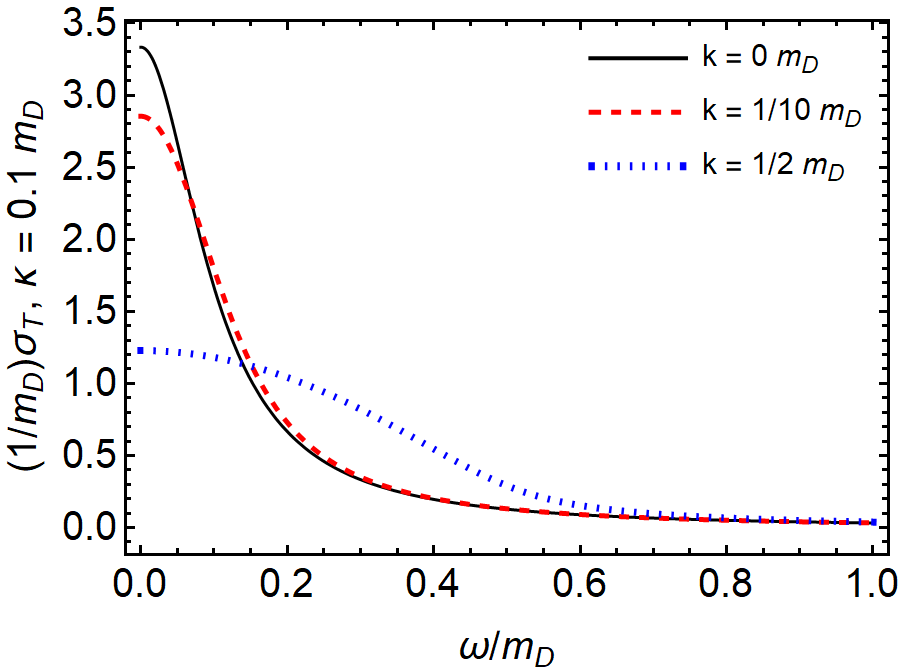
\includegraphics[width=0.95\linewidth]{plots/chap01intro/condtRe.png}
% 	\caption{Real part of $\sigma_T$ for different values of $k$.}
% 	\label{fig:sigma_T}
% \end{figure}
% The conductivity tensor is commonly defined by the spatial part of the linear response equation (\ref{eq:ohm}), where the vector potential is expressed in terms of the electric field $i \omega \widetilde{A^i} = \widetilde{E^i}$. One finds Refs.~\cite{Starke:2014tfa,melrose2008quantum}:
% \begin{align}
%     \sigma_T(\omega,k) &\equiv - i \omega \chi_T(\omega, k)\,,\\
%     \sigma_L(\omega,k) &\equiv - i \omega \chi_L(\omega, k)\,.
% \end{align}
% We only consider the real part of the conductivity for the two independent response functions ($\Pi_L$) and ($\Pi_T$), which are shown in Figs.~\ref{fig:sigma_L} and \ref{fig:sigma_T} for three different values of $k$. 
% Looking at the $k \to 0$ limit of the transverse susceptibility in equation (\ref{chi_l_opt}), we see that the transverse and longitudinal conductivities have the same Drude model dependence on frequency~\cite{Drude:1900} with $\tau = 1/\kappa$:
% \begin{equation}
%     \sigma_L(\omega,0) = \sigma_T(\omega,0) = \frac{\omega_p^2\tau}{1-i \omega\tau} \,,
% \end{equation}
% which reproduces Satow's gradient expansion~\cite{Satow:2014lia}. We note the discontinuous behavior of longitudinal conductivity
% \begin{equation}
% \lim_{k\rightarrow 0}\sigma_L(0,k) \neq \lim_{\omega\rightarrow 0}\sigma_L(\omega,0)\,,
% \end{equation}
% which originates in the infinite extent of the plasma considered in this work. For finite systems, the longitudinal conductivity vanishes in the limit $\omega \rightarrow 0$ even in the $k = 0$ case \cite{Baranger:1989elt}.
% %==================================================================================
% \subsection{Dispersion Relations} \label{sec:disp}

% The propagator of electromagnetic perturbations of the plasma is obtained by inverting Maxwell's equations including the induced current:
% \begin{equation}
%     -ik_{\mu}\widetilde{F}^{\mu \nu} = \mu_0( \widetilde{j}_{\mathrm{ind}}^{\nu}+\widetilde{j}_{\mathrm{ext}}^{\nu})
% \end{equation}
% Including the induced current on the left-hand side of the equation and writing the expression in-terms of $A^{\mu}$ one finds,
% \begin{equation}
%     (k^2g^{\mu \nu} - k^{\mu} k^{\nu} + \mu_0\Pi^{\mu \nu})\widetilde{A}_{\nu} = - \mu_0\widetilde{j}_{\mathrm{ext}}^{\nu} \,.
% \end{equation}
% The propagator $D^\mu_\nu(k)$ is obtained by inverting the equation:
% \begin{equation}
%     \widetilde{A}_{\nu}(k) = -D^{\mu}_{\nu}(k) \,\widetilde{j}_{\mathrm{ext}}^{\nu}(k) \,.
% \end{equation}
% For an isotropic medium the poles in the propagator can be expressed in terms of $\Pi_L$ and $\Pi_T$; the result is~\cite{melrose2008quantum}:
% \begin{equation}
% \left[(k\cdot u)^2+ \mu_0\Pi_L(\omega, k)\right]\left[k^2 + \mu_0 \Pi_T(\omega, k)\right]^2=0 \,,
% \end{equation}
% where again $u$ is the 4-velocity of the medium rest frame. Note that the transverse mode has duplicate solutions as it describes modes in a plane perpendicular to $k$.

% In the limit of $k \to 0$ both the transverse and longitudinal roots of the dispersion relation reduce to the frequency of plasma oscillations (Figure \ref{fig:plasma-freq}):
% \begin{equation}\label{plasmafreq}
%     \omega_{\pm} = -\frac{i\kappa}{2} \pm \sqrt{\omega_p^2 - \frac{\kappa}{4}^2}\,,
% \end{equation}
% where the plasma frequency $\omega_p$ is explicitly given in the ultrarelativistic and non-relativistic limits, respectively, by:
% \begin{equation}
% \omega_p^2 = \frac{1}{3} m_D^2 \quad (\mathrm{UR})\,, \qquad \omega_p^2 = m_L^2 \quad (\mathrm{NR}) \,.
% \end{equation}
% This expression gives a physical meaning to the mass $m_L$ introduced in (\ref{eq:mL}).

% For oscillatory waves of the form $E=E_0e^{-i\omega t}$, in the case of $\kappa \ll \omega_p$ the waves are weakly damped. For $\kappa > 2\omega_p$, the square root is imaginary and the wave becomes overdamped. For $\kappa \gg \omega_p$ the weakly damped solution has a long lifetime $\tau \approx \kappa/\omega_p^2$. The plasma frequency is plotted below as a function of $\kappa$.
% \begin{figure}
%     \centering
%     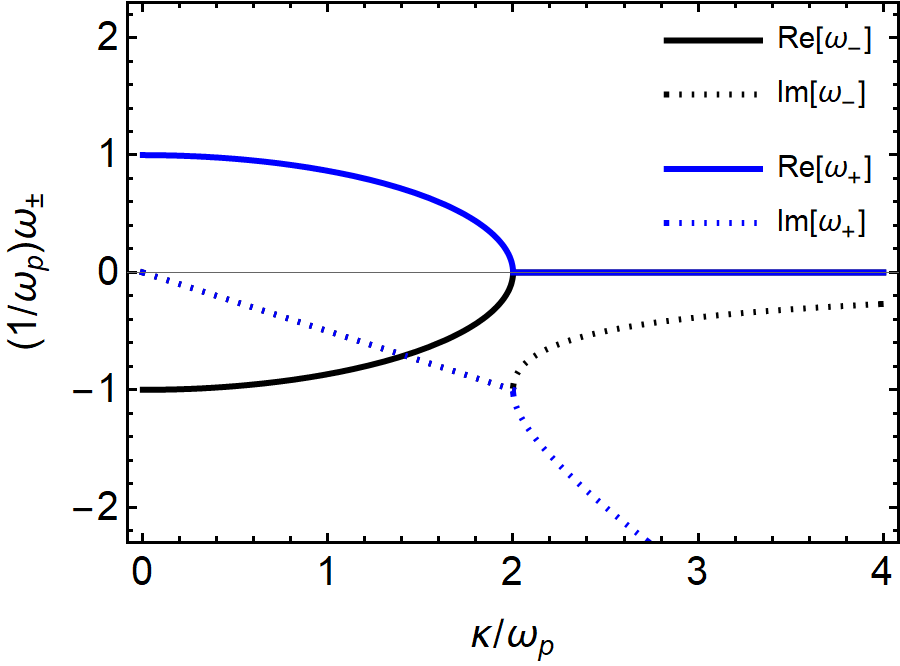
\includegraphics[width=0.95\linewidth]{plots/chap01intro/plasma.png}
%     \caption{Real and imaginary part of the plasma frequencies $\omega_\pm$ as a function of $\kappa$. 
%     The region $\kappa>2\omega_p$ corresponds to overdamping, with one mode becoming more quickly damped 
%     and the other more slowly damped.}
%     \label{fig:plasma-freq}
% \end{figure}

% In the static limit $\omega \rightarrow 0$ the solutions to the longitudinal root of the dispersion relation go to
% \begin{equation}
%     k = \pm  i m_D \,.
% \end{equation}
% The positive imaginary root describes the Debye screening of a stationary charge within the plasma. The analysis of the real and imaginary parts of the zeros for the $\kappa$-dependent dispersion relation for both transverse and longitudinal modes can be found in \cite{Carrington:2003je,Schenke:2006xu}. Our approach starting from manifestly covariant formulation with arbitrary medium 4-velocity matches these results.


% %=======================================================================

% %===================================================================
% \subsection{Ultrarelativistic limit}\label{sec:ultrarel}
% \textcolor{blue}{these are appendix topics decide how to include}
% For the calculation of the components of the polarization tensor (\ref{eq:pimunu}) we consider the rest frame of the medium $u^\mu = (c,0)$ and the massless limit of particles moving at the speed of light
% \begin{align}
% \label{eq:massless1}p^\mu &= |\pmb{p}|v^\mu,\\
%  v^\mu &= (1, \sin\theta\cos\varphi, \sin\theta\sin\varphi,\cos\theta)\,.
% \end{align}
% That way the product $p \cdot u$ can be expressed as
% \begin{equation}
% \label{eq:massless2}p \cdot u = p^0 = |\pmb{p}|\,.
% \end{equation}
% Without loss of generality we choose to orient the $\pmb{k}$ vector along the $z$-axis. That way the covariant $k^\mu$ reads
% \begin{equation}
% \label{eq:kdirect}k^\mu = (\omega, 0,0,k)\,.
% \end{equation}
% the product $p \cdot k$ is given by
% \begin{equation}
% p \cdot k = |\pmb{p}|(\omega - k \cos \theta)\,.
% \end{equation}
% For example the $n_\mathrm{eq}$ integral (\ref{eq:ndef2}) in the approximation of mass-less particles
% \begin{equation}
% n_\mathrm{eq} = \frac{1}{\pi^2}\int_0^\infty |\pmb{p}|^2d|\pmb{p}| f_\mathrm{eq}(|\pmb{p}|) = \frac{3T^3}{2\pi^2}\zeta(3)\,, 
% \end{equation}
% because the angular integration in the rest frame of the medium is trivial.
% %===================================================================
% \subsection{Evaluating $R^\mu_\nu(k)$}
% The definition of $R^\mu_\nu(k)$ is given in (\ref{eq:Rmunu}). Under the conditions described above (\ref{eq:massless1}-\ref{eq:kdirect}) we have
% \begin{equation}
% 	R^\mu_\nu = -2q^2\int_0^\infty \frac{|\pmb{p}|^2d|\pmb{p}|}{\pi^2 }f'_\mathrm{eq}(|\pmb{p}|)
% 	\times \int \frac{d\Omega}{4\pi}\frac{\omega v^\mu v_\nu - (\omega - k \cos \theta)v^\mu \delta_{\nu 0}}{\omega - k \cos \theta + i\kappa}\,.
% \end{equation}
% We see that the integrals over the magnitude of momentum and the angular integrals in this limit separated. The integral over the magnitude is customarily called Debye screening mass
% \begin{equation}\label{eq:mD}
% m_D^2 \equiv - \frac{2q^2}{\pi^2}\int_0^\infty |\pmb{p}|^2d|\pmb{p}| f'_\mathrm{eq}(|\pmb{p}|) = \frac{q^2T^2}{3}\,.
% \end{equation}
% The angular integration eliminates most of the tensor components. The only non-zero terms are
% \begin{align}
% 	\label{eq:r00}R^0_0 &= - m_D^2 L\,,\\
% 	R^x_x = R^y_y &= \frac{m_D^2\omega}{4k} \left(\frac{\omega'^2}{k^2}\Lambda - \Lambda - \frac{2\omega'}{k}\right)\,,\\
% 	\label{eq:r0z}R^0_z &=  m_D^2\frac{\omega}{k}L\,,\\
% 	R^z_0 & = - m_D^2\frac{\omega'}{k}L\,,\\
% 	\label{eq:rzz}R^z_z &= m_D^2\frac{\omega \omega'}{k^2}L\,,
% \end{align}
% where the quantities $\omega'$, $\Lambda$, and $L$ are defined in (\ref{eq:definitions}).

% %===================================================================
% \subsection{Evaluating $Q(k)$}

% The scalar term $Q(k)$ (\ref{eq:Q}) can be also split into integration over the magnitude of momentum and angular part under conditions (\ref{eq:massless1}-\ref{eq:kdirect})
% \begin{equation}
% 	Q(k) = - i \frac{\kappa}{n_\mathrm{eq}} \int_0^\infty \frac{|\pmb{p}|^2d|\pmb{p}|}{\pi^2}f_\mathrm{eq}(|\pmb{p}|)
% 	\times\frac{1}{4\pi}\int\frac{d\Omega}{\omega - k\cos\theta + i\kappa}\,. 
% \end{equation}
% The integral over the magnitude of $|\pmb{p}|$ reads
% \begin{equation}
% - \frac{i}{\pi^2} \frac{\kappa}{n_\mathrm{eq}} \int_0^\infty |\pmb{p}|^2d|\pmb{p}|f_\mathrm{eq}(|\pmb{p}|) = -i\kappa\,,
% \end{equation}
% where the dependence on $n_\mathrm{eq}$ exactly cancelled. The angular integral is
% \begin{equation}
% \frac{1}{4\pi}\int\frac{d\Omega}{\omega - k\cos\theta + i\kappa} = \frac{1}{2k}\Lambda\,.
% \end{equation}
% Altogether we have for $Q(k)$
% \begin{equation}\label{eq:qres}
% \boxed{Q(k) = -\frac{i\kappa}{2k}\Lambda\,.}
% \end{equation}

% %===================================================================
% \subsection{Evaluating $Q^\mu(k)$}

% Repeating the same logic for the $Q^\mu(k)$ term (\ref{eq:Qmu}) we have
% \begin{equation}
% 	Q^\mu(k) = - 2qi \frac{\kappa}{n_\mathrm{eq}} \int_0^\infty \frac{|\pmb{p}|^2d|\pmb{p}|}{\pi^2} f_\mathrm{eq}(|\pmb{p}|)
% 	\times \frac{1}{4\pi}\int \frac{v^\mu d\Omega}{\omega - k \cos \theta + i\kappa}\,.
% \end{equation}
% The integral over the magnitude $|\pmb{p}|$ is
% \begin{equation}
% - \frac{2qi}{\pi^2} \frac{\kappa}{n_\mathrm{eq}} \int_0^\infty |\pmb{p}|^2d|\pmb{p}|f_\mathrm{eq}(|\pmb{p}|) = - 2iq\kappa\,,
% \end{equation}
% where again the $\zeta(3)T^3$ dependence of $n_\mathrm{eq}$ cancelled. The nonzero contributions of the angular part are
% \begin{align}
% 	I^0 = \frac{1}{4\pi}\int \frac{d\Omega}{\omega - k\cos\theta + i\kappa} &= \frac{1}{2k}\Lambda\,,\\
% 	I^z = \frac{1}{4\pi}\int \frac{\cos \theta d\Omega}{\omega - k\cos\theta + i\kappa}& = - \frac{1}{k}L\,.
% \end{align}
% Therefore the non-zero components of $Q^\mu(k)$ are
% \begin{equation}\label{eq:qmures}
% \boxed{Q^0 =- \frac{iq\kappa}{k}\Lambda, \quad Q^z = \frac{2iq\kappa}{k}L\,.}
% \end{equation}
% %===================================================================
% \subsection{Evaluating $H_\nu(k)$}

% Separating the itegration into the angular and magnitude part from the definition of $H_\nu$ (\ref{eq:Hnu}) we have
% \begin{equation}
% 	H_\nu(k) = - q \int_0^\infty \frac{|\pmb{p}|^2 d|\pmb{p}|}{\pi^2}f'_\mathrm{eq}(|\pmb{p}|)
% 	\times \int \frac{d\Omega}{4\pi} \frac{\omega v_\nu - (\omega - k\cos\theta)\delta_{\nu 0}}{\omega - k \cos \theta + i\kappa}\,.
% \end{equation}
% The integral over magnitude $|\pmb{p}|$ is
% \begin{equation}
% -\frac{q}{\pi^2}\int_0^\infty |\pmb{p}|^2d|\pmb{p}|f'_\mathrm{eq}(|\pmb{p}|)= \frac{qT^2}{6}
% \end{equation}
% and the angular integral has only two non-zero components
% \begin{align}
% 	I_0 &= \int \frac{d\Omega}{4\pi} \frac{k\cos\theta}{\omega-k\cos\theta+i\kappa}= - L\,,\\
% 	I_z &= -\int \frac{d\Omega}{4\pi} \frac{\omega \cos \theta}{\omega - k\cos \theta + i \kappa} = \frac{\omega}{k}L\,.
% \end{align}
% The change in sign is due to $v_z = - \cos\theta$ because of the lowered index. Altogether the non-zero components of $H_\nu(k)$ are
% \begin{equation}\label{eq:hnures}
% \boxed{H_0 = -\frac{qT^2}{6}L, \quad H_z = \frac{qT^2 \omega}{6 k}L\,.}
% \end{equation}

% %=====================================================================
% \subsection{Summary of the components}

% Using the results (\ref{eq:r00}-\ref{eq:rzz}) and (\ref{eq:qres},\ref{eq:qmures},\ref{eq:hnures}) the components of the polarization tensor (\ref{eq:pimunu}) are
% \begin{align}
% 	\label{eq:pi00}\Pi^0_0  &= - m_D^2 L \left( 1+ \frac{i\kappa\Lambda}{2k-i\kappa\Lambda} \right)\,,\\
% 	\label{eq:pi0z}\Pi^0_z &=m_D^2 \frac{\omega}{k}L \left( 1+ \frac{i\kappa\Lambda}{2k-i\kappa\Lambda} \right)\,,\\
% 	\label{eq:piz0}\Pi^z_0 &= - m_D^2 L \left( \frac{\omega'}{k} - \frac{2i\kappa L}{2k-i\kappa\Lambda} \right)\,,\\
% 	\label{eq:pizz}\Pi^z_z &= m_D^2 \frac{\omega}{k}L \left( \frac{\omega'}{k} - \frac{2i\kappa L}{2k-i\kappa\Lambda} \right)\,.
% \end{align}
% Additionally the transversal components are given just by $R^\mu_\nu$
% \begin{equation}
% \Pi^x_x = \Pi^y_y = \frac{m_D^2\omega}{4k}\left( \frac{\omega'^2}{k^2}\Lambda - \Lambda - \frac{2\omega'}{k}\right)\,.
% \end{equation} 
% The gauge invariance conditions (\ref{eq:gaugeincomponents}) are obviously satisfied. In order to prove the current conservation condition (\ref{eq:currentconservcomp}) we need to combine the $i\kappa$ proportional term from $\omega'$ in the first term in (\ref{eq:piz0}) with the second term and recover the second term in (\ref{eq:pi00}) times $\omega/k$
% \begin{equation}
% 	\frac{i\kappa}{k} - \frac{2i\kappa L}{2k - i\kappa \Lambda} = \frac{\kappa^2 \Lambda + i \kappa \omega' \Lambda}{k(2k-i\kappa \Lambda)} =\frac{\omega}{k} \frac{i\kappa \Lambda}{2k-i\kappa \Lambda)}\,.
% \end{equation}
% In the first step we substituted the definition of $L$ (\ref{eq:definitions}) and in the second step the $i\kappa$ part of $\omega'$ in the numerator cancels and we obtain $\omega/k$ times the second term of (\ref{eq:pi00}) as expected. This also means that the last two components of $\Pi^\mu_\nu$ (\ref{eq:piz0},\ref{eq:pi0z}) can be written equivalently as
% \begin{align}
% 	\Pi^z_0 &= -m_D^2\frac{\omega}{k}L\left(1 + \frac{i\kappa \Lambda}{2k - i\kappa \Lambda}\right)\,,\\
% 	\Pi^z_z &= m_D^2\frac{\omega^2}{k^2}L\left(1 + \frac{i\kappa \Lambda}{2k - i\kappa \Lambda}\right)\,.
% \end{align}
% In this form we see explicitly that baring the lowering of the spatial index
% \begin{equation}\label{eq:symmetry}
% \Pi^0_z = -\Pi^z_0\,.
% \end{equation}
% the tensor $\Pi_{\mu\nu}$ is symmetric. 

% %===================================================================
% \subsection{Relativistic Expansion}\label{sec:nonrel}
% \subsection{Non-relativistic limit}\label{sec:nonrel}

% We now consider the low-temperature non-relativistic limit. For low temperatures ($T \ll m$) the Fermi distribution can be replaced by the Boltzmann factor
% \begin{equation}
% f_\mathrm{eq} \approx \exp\left(- \frac{p \cdot u}{T}\right)
% \end{equation}
% and in the non-relativistic limit we approximate the energy in the rest frame by its nonrelativistic expansion
% \begin{equation}
% (p \cdot u) = p^0 = m \left(1 + \frac{|\pmb{p}|^2}{2m^2} + \ldots \right)\,.
% \end{equation}
% In the following we will keep only the first term of this expansion. For example we can evaluate the $n_\mathrm{eq}$ integral (\ref{eq:ndef2}) as
% \begin{equation}
% n_{eq} = \int \frac{d\Omega}{4\pi}\frac{|\pmb{p}|^2d|\pmb{p}|}{\pi^2}\exp\left[-\frac{m}{T}\left(1 + \frac{1}{2}\frac{|\pmb{p}|^2}{m^2}\right)\right]\,.
% \end{equation}
% The angular integration is trivial and the rest gives us a gaussian integral
% \begin{equation}
% n_\mathrm{eq} = \frac{1}{4}e^{-m/T}\left(\frac{2mT}{\pi} \right)^{3/2}\,.
% \end{equation}
% The denominator of all the integrals reads
% \begin{equation}
% p \cdot k + i(p \cdot u)\kappa = p^0\left(\omega - \frac{|\pmb{p}|}{p^0}k\cos \theta +i\kappa\right)
% \end{equation}
% and in the first order 
% \begin{equation}
% \frac{|\pmb{p}|}{p^0} \approx \frac{|\pmb{p}|}{m}\,.
% \end{equation}
% Unfortunately, as we will see below, the angular and magnitude integration no longer factorize. We will resolve this problem by computing all angular integrals up to the quadratic order in the small parameter $|\pmb{p}|/m$.

% %===================================================================
% \subsection{Evaluation of $R^\mu_\nu(k)$}

% The definition of $R^\mu_\nu(k)$ is given in (\ref{eq:Rmunu}). In non-relativistic and low-temperature limit we have
% \begin{equation}
% 	R^\mu_\nu(k) = -2q^2 \int_0^\infty \frac{|\pmb{p}|^2 d|\pmb{p}|}{\pi^2}f'_\mathrm{eq}(|\pmb{p}|)
% 	\times \frac{1}{p^0}\int \frac{d\Omega}{4\pi} \frac{\omega p^\mu p_\nu - (k \cdot p)p^\mu \delta_{0\nu}}{k \cdot p+ i(p \cdot u)\kappa}\,.
% \end{equation}
% Introducing the abbreviation
% \begin{equation}
% g(\cos\theta) = \omega -|\pmb{p}|k\cos\theta / m + i\kappa \,,
% \label{eq:dcostheta}
% \end{equation}
% the angular integrals are easily evaluated in up to quadratic order of $|\pmb{p}|/m$:
% \begin{align}
% 	I^0_0 &= \int \frac{d\Omega}{4\pi} \frac{|\pmb{p}|k\cos\theta}{g(\cos\theta)m} \approx
% 	\frac{1}{3}\left(\frac{|\pmb{p}|k}{m\omega'}\right)^2\,,\\
% 	I^0_z &= - \int \frac{d\Omega}{4\pi} \frac{\omega |\pmb{p}|\cos\theta}{g(\cos\theta)m} \approx - \frac{1}{3}\frac{\omega|\pmb{p}|^2k}{\omega'^2m^2}\,,\\
% 	I^z_0 &= \int \frac{d\Omega}{4\pi}\frac{|\pmb{p}|^2 k \cos^2\theta}{g(\cos\theta)m^2} \approx \frac{1}{3} \frac{|\pmb{p}|^2 k}{\omega' m^2}\,,\\
% 	I^z_z &= - \int \frac{d\Omega}{4\pi} \frac{|\pmb{p}|^2 \omega \cos^2\theta}{g(\cos\theta)m^2} \approx - \frac{1}{3}\frac{|\pmb{p}|^2\omega}{m^2 \omega'}\,,\\
% 	I^x_x &= I^y_y = - \int \frac{d\Omega}{4\pi} \frac{\omega |\pmb{p}|^2 \sin^2\theta \cos^2 \varphi}{g(\cos\theta)m^2} \approx - \frac{1}{3}\frac{|\pmb{p}|^2\omega}{m^2 \omega'}\,.
% \end{align}
% In order for the expansion to be possible $|\pmb{p}|k/m\omega' \ll 1$ which places also limit on $k$ and $\omega'$. All the magnitude integrals are now of the type
% \begin{equation}\label{eq:mL}
% 	m_L^2 \equiv \frac{2q^2}{3m^2\pi^2}\int_0^\infty |\pmb{p}|^4 d|\pmb{p}| \left(\frac{1}{T} e^{-p^0/T} \right)
% 	= q^2 \left(\frac{2mT}{\pi}\right)^{3/2}\frac{e^{-m/T}}{2m}\,,
% \end{equation}
% where $m_L^2$ defines a mass scale. Altogether
% \begin{equation}\label{eq:r00nonrel}
% R^0_0 = m_L^2 \frac{k^2}{\omega'^2}\,, \quad R^0_z = -m_L^2 \frac{\omega k}{\omega'^2}\,,
% \end{equation}
% \begin{equation}\label{eq:rz0nonrel}
% R^z_0 = m_L^2 \frac{k}{\omega'}\,, \quad R^x_x = R^y_y = R^z_z = -m_L^2 \frac{\omega}{\omega'}\,.
% \end{equation}

% %===================================================================
% \subsection{Evaluation of $Q(k)$}

% In the low temperature and non-relativistic limit the integral for $Q(k)$ (\ref{eq:Q}) becomes
% \begin{equation}
% 	Q(k) = -i \frac{\kappa}{n_\mathrm{eq}} \int_0^\infty \frac{|\pmb{p}|^2d|\pmb{p}|}{\pi^2} f_\mathrm{eq}(|\pmb{p}|) 
% 	\times \int \frac{d\Omega}{4\pi} \frac{1}{\omega - |\pmb{p}|k \cos \theta/m +i\kappa}\,,
% \end{equation}
% in which again the integrals over angles and magnitude of the momentum $\pmb{p}$ not quite separate. Up to quadratic terms in $|\pmb{p}|/m$ the angular integral is
% \begin{equation}
% \int \frac{d\Omega}{4\pi} \frac{1}{g(\cos\theta)} \approx \frac{1}{\omega'}\left(1 + \frac{1}{3}\frac{|\pmb{p}|^2k^2}{m^2 \omega'^2}\right)\,,
% \end{equation}
% giving the result:
% \begin{equation}\label{eq:qnonrel}
% \boxed{Q(k) = -\frac{i\kappa}{\omega'} \left(1 + \frac{T k^2}{m\omega'^2} \right)\,.}
% \end{equation}

% %===================================================================
% \subsection{Evaluation of $Q^\mu(k)$}

% In the low temperature and non-relativistic limit the integral for $Q^\mu(k)$ (\ref{eq:Qmu}) becomes
% \begin{equation}
% 	Q^\mu(k) = -2qi \frac{\kappa}{n_\mathrm{eq}} \int_0^\infty \frac{|\pmb{p}|^2d|\pmb{p}|}{\pi^2} f_\mathrm{eq}(|\pmb{p}|)	
% 	\times \int \frac{d\Omega}{4\pi} \frac{p^\mu/m}{\omega - |\pmb{p}|k\cos\theta / m + i \kappa}\,,
% \end{equation}
% where the only non-zero angular integrals are up to second order in $|\pmb{p}|/k$
% \begin{align}
% 	I^0 &= \int \frac{d\Omega}{4\pi} \frac{1}{g(\cos\theta)} \approx \frac{1}{\omega'} + \frac{1}{3} \frac{|\pmb{p}|^2 k^2}{m^2 \omega'^3}\,,\\
% 	I^z &= \int \frac{d\Omega}{4\pi} \frac{|\pmb{p}|\cos\theta}{g(\cos\theta)m} \approx \frac{1}{3} \frac{|\pmb{p}|^2k}{m^2 \omega'^2}\,.
% \end{align}
% Finally, after integration over the magnitude we have for the two non-zero components of $Q^\mu(k)$
% \begin{equation}\label{eq:qmunonrel}
% \boxed{Q^0 = - \frac{2qi\kappa}{\omega'}\left(1 + \frac{T k^2}{m\omega'^2} \right)\,, \quad Q^z = -2qi\kappa \frac{T k}{m\omega'^2}\,.}
% \end{equation}

% %===================================================================
% \subsection{Evaluation of $H_\nu(k)$}

% In the low temperature and non-relativistic limit the integral for $H_\nu(k)$ (\ref{eq:Hnu}) becomes
% \begin{equation}
% 	H_\nu(k) = - q \int_0^\infty \frac{|\pmb{p}|^2d|\pmb{p}|}{\pi^2} f'_\mathrm{eq}(|\pmb{p}|) 
% 	\times \frac{1}{p^0} \int \frac{d\Omega}{4\pi} \frac{\omega p_\nu - (k \cdot p) \delta_{0\nu}}{\omega - |\pmb{p}|k\cos\theta / m + i\kappa}\,.
% \end{equation}
% The only non-zero angular integrals up to the second order in $|\pmb{p}|/k$ read
% \begin{align}
% 	I_0 &= \int \frac{d\Omega}{4\pi} \frac{|\pmb{p}|k\cos\theta}{g(\cos\theta)m} \approx \frac{1}{3}\left(\frac{|\pmb{p}|k}{m\omega'}\right)^2\,,\\
% 	I_z &= - \int \frac{d\Omega}{4\pi} \frac{\omega|\pmb{p}|\cos\theta}{g(\cos\theta)m} \approx - \frac{1}{3} \frac{\omega |\pmb{p}|^2 k}{m^2 \omega'^2}\,.
% \end{align}
% After integration over $|\pmb{p}|$ we have two non-zero components of $H_\nu(k)$
% \begin{equation}\label{eq:hnunonrel}
% \boxed{H_0 = \frac{1}{2q} m_L^2 \frac{k^2}{\omega'^2}\,, \quad H_z = -\frac{1}{2q} m_L^2 \frac{\omega k}{\omega'^2}\,.}
% \end{equation}

% %===================================================================
% \subsection{Polarization tensor}

% If we substitute the results obtained in the non-relativistic and low temperature limit (\ref{eq:r00nonrel},\ref{eq:rz0nonrel},\ref{eq:qnonrel},\ref{eq:qmunonrel},\ref{eq:hnunonrel}) back into (\ref{eq:pimunu}) we obtain the following expressions for the components of the polarization tensor
% \begin{align}
% 	\Pi^0_0 &= m_L^2 \frac{k^2}{\omega'^2} \frac{1}{1-\frac{i\kappa}{\omega'}\left(1+\frac{T k^2}{m\omega'^2} \right)}\,,\\
% 	\label{eq:pi0znonrel}\Pi^0_z &= -m_L^2 \frac{\omega k}{\omega'^2} \frac{1}{1-\frac{i\kappa}{\omega'}\left(1+\frac{T k^2}{m\omega'^2} \right)}\,,\\
% 	\label{eq:piz0nonrel}\Pi^z_0 &= m_L^2 \frac{k^2}{\omega'^2} \left[\frac{\omega'}{k} + \frac{i\kappa\frac{T k}{m\omega'^2}}{1-\frac{i\kappa}{\omega'}\left(1+\frac{T k^2}{m\omega'^2} \right)} \right]\,,\\
% 	\label{eq:pizznonrel}\Pi^z_z &= -m_L^2 \frac{\omega k}{\omega'^2} \left[\frac{\omega'}{k} + \frac{i\kappa\frac{T k}{m\omega'^2}}{1-\frac{i\kappa}{\omega'}\left(1+\frac{T k^2}{m\omega'^2} \right)} \right]\,,\\	
% 	\Pi^x_x &= \Pi^y_y = -m_L^2 \frac{\omega}{\omega'}\,.	
% \end{align}
	
% The gauge conditions for the components (\ref{eq:gaugeincomponents}) are again obviously satisfied. The current conservation condition in components (\ref{eq:currentconservcomp}) requires further attention. Let's put the term in the parentheses of (\ref{eq:piz0nonrel}) on a common denominator and evaluate the numerator
% \begin{equation}
% 	\frac{\omega'}{k}\left[1-\frac{i\kappa}{\omega'}\left(1+\frac{T k^2}{m\omega'^2} \right)\right] + i \kappa \frac{T k}{m\omega'^2}
% 	= \frac{\omega}{k} + \frac{i\kappa}{k}\left(1 + \frac{T k^2}{m\omega'^2}\right) - \frac{i\kappa}{k}\left(1 + \frac{T k^2}{m\omega'^2}\right) = \frac{\omega}{k}\,,
% \end{equation}
% as we were supposed to get. Therefore (\ref{eq:piz0nonrel}) and (\ref{eq:pizznonrel}) can be equivalently rewritten as
% \begin{align}
% 	\Pi^z_0 &= m_L^2 \frac{\omega k}{\omega'^2} \frac{1}{1-\frac{i\kappa}{\omega'}\left(1+\frac{T k^2}{m\omega'^2} \right)}\,,\\	
% 	\Pi^z_z &= -m_L^2 \frac{\omega^2}{\omega'^2} \frac{1}{1-\frac{i\kappa}{\omega'}\left(1+\frac{T k^2}{m\omega'^2} \right)}\,.
% \end{align}

% \vspace*{0.1in}


%%%%%%%%%%%%%%%%%%%%%%%%%%%%%%%%%%%%%%%%%%%%%%%%%%%
%%%%%%%%%%%%%%%%%%%
% \begin{thebibliography}{66}
	
% 	\bibitem{NAS_HED:2003}
% 	National Research Council, 
% 	{\it Frontiers in High Energy Density Physics: The X-Games of Contemporary Science}, 
% 	(The National Academies Press, Washington, DC, 2003). 
% 	%doi:10.17226/10544
	
% 	\bibitem{DOE-BRN:2009}
% 	{\it Report of the Workshop on High Energy Density Laboratory Research Needs},
% 	U.S. Department of Energy, Office of Science and National Nuclear Security Administration,
% 	November 15-18, 2009.

% 	\bibitem{Weldon:1982aq}
% 	H.~A.~Weldon,
% 	%\lq\lq Covariant Calculations at Finite Temperature: The Relativistic Plasma,\rq\rq
% 	Phys. Rev. D \textbf{26}, 1394 (1982).
% 	%doi:10.1103/PhysRevD.26.1394
	
% 	%\cite{}
% 	\bibitem{Mrowczynski:1987jr}
% 	S.~Mr\'owczy\'nski,
% 	%``SMALL OSCILLATIONS OF A COLLISIONLESS QUARK PLASMA,''
% 	Phys. Lett. B \textbf{188}, 129 (1987).
% 	%doi:10.1016/0370-2693(87)90718-0
	
% 	\bibitem{Mrowczynski:1989np}
% 	S.~Mr\'owczy\'nski,
% 	%``KINETIC THEORY APPROACH TO QUARK - GLUON PLASMA OSCILLATIONS,''
% 	Phys. Rev. D \textbf{39}, 1940 (1989).
% 	%doi:10.1103/PhysRevD.39.1940
	
% 	\bibitem{Blaizot:1993zk}
% 	J.~P.~Blaizot and E.~Iancu,
% 	%``Kinetic equations for long wavelength excitations of the quark - gluon plasma,''
% 	Phys. Rev. Lett. \textbf{70}, 3376 (1993)
% 	%doi:10.1103/PhysRevLett.70.3376
% 	[arXiv:hep-ph/9301236 [hep-ph]].
	
% 	\bibitem{Kelly:1994ig}
% 	P.~F.~Kelly, Q.~Liu, C.~Lucchesi and C.~Manuel,
% 	%``Deriving the hard thermal loops of QCD from classical transport theory,''
% 	Phys. Rev. Lett. \textbf{72}, 3461 (1994)
% 	%doi:10.1103/PhysRevLett.72.3461
% 	[arXiv:hep-ph/9403403 [hep-ph]].
	
% 	\bibitem{Kelly:1994dh}
% 	P.~F.~Kelly, Q.~Liu, C.~Lucchesi and C.~Manuel,
% 	%``Classical transport theory and hard thermal loops in the quark - gluon plasma,''
% 	Phys. Rev. D \textbf{50}, 4209 (1994)
% 	%doi:10.1103/PhysRevD.50.4209
% 	[arXiv:hep-ph/9406285 [hep-ph]].
	
% 	\bibitem{Blaizot:2001nr}
% 	J.~P.~Blaizot and E.~Iancu,
% 	%``The Quark gluon plasma: Collective dynamics and hard thermal loops,''
% 	Phys. Rept. \textbf{359}, 355 (2002)
% 	%doi:10.1016/S0370-1573(01)00061-8
% 	[arXiv:hep-ph/0101103 [hep-ph]].
		
% 	\bibitem{Mrowczynski:1988xu}
% 	S.~Mr\'owczy\'nski,
% 	%``On the Transport Coefficients of a Quark Plasma,''
% 	Acta Phys. Polon. B \textbf{19}, 91 (1988).
% 	%\cite{Ahonen:1998iz}
	
% 	\bibitem{Heiselberg:1993cr}
% 	H.~Heiselberg and C.~J.~Pethick,
% 	%``Transport and relaxation in degenerate quark plasmas,''
% 	Phys. Rev. D \textbf{48}, 2916 (1993).
% 	%doi:10.1103/PhysRevD.48.2916
	
% 	\bibitem{Ahonen:1996nq}
% 	J.~Ahonen and K.~Enqvist,
% 	%``Electrical conductivity in the early universe,''
% 	Phys. Lett. B \textbf{382}, 40 (1996)
% 	%doi:10.1016/0370-2693(96)00633-8
% 	[arXiv:hep-ph/9602357 [hep-ph]].
	
% 	\bibitem{Baym:1997gq}
% 	G.~Baym and H.~Heiselberg,
% 	%``The Electrical conductivity in the early universe,''
% 	Phys. Rev. D \textbf{56}, 5254 (1997)
% 	%doi:10.1103/PhysRevD.56.5254
% 	[arXiv:astro-ph/9704214 [astro-ph]].
	
% 	\bibitem{Ahonen:1998iz}
% 	J.~Ahonen,
% 	%``Transport coefficients in the early universe,''
% 	Phys. Rev. D \textbf{59}, 023004 (1999)
% 	%doi:10.1103/PhysRevD.59.023004
% 	[arXiv:hep-ph/9801434 [hep-ph]].
	
% 	\bibitem{Heiselberg:1994ms}
% 	H.~Heiselberg,
% 	%``Transport properties of quark and gluon plasmas,''
% 	[arXiv:hep-ph/9401300 [hep-ph]].
	
% 	\bibitem{Arnold:2002zm}
% 	P.~B.~Arnold, G.~D.~Moore and L.~G.~Yaffe,
% 	%``Effective kinetic theory for high temperature gauge theories,''
% 	JHEP \textbf{01}, 030 (2003)
% 	%doi:10.1088/1126-6708/2003/01/030
% 	[arXiv:hep-ph/0209353 [hep-ph]].
	
% 	\bibitem{Arnold:2003zc}
% 	P.~B.~Arnold, G.~D.~Moore and L.~G.~Yaffe,
% 	%``Transport coefficients in high temperature gauge theories. 2. Beyond leading log,''
% 	JHEP \textbf{05}, 051 (2003)
% 	%doi:10.1088/1126-6708/2003/05/051
% 	[arXiv:hep-ph/0302165 [hep-ph]].
	
% 	\bibitem{Satow:2014lia}
% 	D.~Satow,
% 	%\lq\lq Nonlinear electromagnetic response in quark-gluon plasma,\rq\rq
% 	Phys. Rev. D \textbf{90}, 034018 (2014)
% 	%doi:10.1103/PhysRevD.90.034018
% 	[arXiv:1406.7032 [hep-ph]].
		
% 	\bibitem{Anderson:1974}
%     	J.~L. Anderson, H.~R. Witting,
%     	%\lq\lq A relativistic relaxation-time model for the Boltzmann equation \rq\rq,
%     	Physica \textbf{74}, 466 (1974).
%     	% https://doi.org/10.1016/0031-8914(74)90355-3.
			
% 	\bibitem{Bhatnagar:1954zz}
% 	P.~L.~Bhatnagar, E.~P.~Gross and M.~Krook,
% 	%``A Model for Collision Processes in Gases. 1. Small Amplitude Processes in Charged and Neutral One-Component Systems,''
% 	Phys. Rev. \textbf{94}, 511 (1954).
% 	%doi:10.1103/PhysRev.94.511
	
% 	\bibitem{Carrington:2003je}
% 	M.~E.~Carrington, T.~Fugleberg, D.~Pickering and M.~H.~Thoma,
% 	%``Dielectric functions and dispersion relations of ultrarelativistic plasmas with collisions,''
% 	Can. J. Phys. \textbf{82}, 671-678 (2004)
% 	%doi:10.1139/p04-035
% 	[arXiv:hep-ph/0312103 [hep-ph]].
	
% 	\bibitem{Schenke:2006xu}
% 	B.~Schenke, M.~Strickland, C.~Greiner and M.~H.~Thoma,
% 	%``A Model of the effect of collisions on QCD plasma instabilities,''
% 	Phys. Rev. D \textbf{73}, 125004 (2006)
% 	%doi:10.1103/PhysRevD.73.125004
% 	[arXiv:hep-ph/0603029 [hep-ph]].

% 	\bibitem{Rocha:2021zcw}
% 	G.~S.~Rocha, G.~S.~Denicol and J.~Noronha,
% 	%``Novel Relaxation Time Approximation to the Relativistic Boltzmann Equation,''
% 	[arXiv:2103.07489 [nucl-th]].
	
% 	%\bibitem{Arnold:1998cy}
% 	%P.~B.~Arnold, D.~T.~Son and L.~G.~Yaffe,
% 	%%``Effective dynamics of hot, soft nonAbelian gauge fields. %Color conductivity and log(1/alpha) effects,''
% 	%Phys. Rev. D \textbf{59}, 105020 (1999)
% 	%doi:10.1103/PhysRevD.59.105020
% 	%[arXiv:hep-ph/9810216 [hep-ph]].
		
% 	\bibitem{Becattini:2013fla}
% 	F.~Becattini, V.~Chandra, L.~Del Zanna and E.~Grossi,
% 	%\lq\lq Relativistic distribution function for particles with spin at local thermodynamical equilibrium,\rq\rq
% 	Annals Phys. \textbf{338}, 32 (2013)
% 	%doi:10.1016/j.aop.2013.07.004
% 	[arXiv:1303.3431 [nucl-th]].
	
% 	\bibitem{Starke:2014tfa}
% 	R.~Starke and G.~A.~H.~Schober,
% 	%\lq\lq Relativistic covariance of Ohm's law,\rq\rq
% 	Int. J. Mod. Phys. D \textbf{25}, 1640010 (2016)
% 	%doi:10.1142/S0218271816400101
% 	[arXiv:1409.3723 [math-ph]].
	
% 	\bibitem{melrose2008quantum}
% 	D.~Melrose,
% 	{\it Quantum Plasmadynamics: Unmagnetized Plasmas},
% 	Lect. Notes Phys. \textbf{735} 
% 	(Springer, New York, 2008).
% 	%doi:10.1007/978-0-387-73903-8
	
% 	\bibitem{Drude:1900}
% 	P.~Drude,
% 	Ann.\ Phys.\ (Leipzig) \textbf{1}, 566 (1900).
	
% 	\bibitem{Baranger:1989}
% 	H.~U.~Baranger, A.~D.~Stone
% 	Phys.\ Rev.\ B \textbf{40}, 8169 (1989).

% \end{thebibliography}


%items to add to bib
% \bibitem{Das:2021bkz}
% A.~Das, H.~Mishra and R.~K.~Mohapatra,
% %``Diffusion matrix associated with the diffusion processes of multiple conserved charges in a hot and dense hadronic matter,''
% Phys. Rev. D \textbf{106} (2022) no.1, 014013
% doi:10.1103/PhysRevD.106.014013
% [arXiv:2109.01543 [nucl-th]].
% %0 citations counted in INSPIRE as of 26 Aug 2022